\documentclass{standalone}
\usepackage{graphicx}
\usepackage{tikz}
\usetikzlibrary{patterns,positioning,calc}
\usepackage{xcolor}

\begin{document}

\definecolor{gt}{HTML}{2E2E2E}
\definecolor{tp}{HTML}{20AEF5}
\definecolor{fp}{HTML}{F5F073}
\newcommand{\ourmodel}{MAD}
\begin{tikzpicture}
    % Define the distance between rows and columns
    \def\colsep{0.24*\textwidth}
    \def\rowsep{1mm}
    \pgfmathsetlengthmacro{\imw}{0.25\textwidth}

    % Titles for columns


    % Draw individual in a grid
    % are 1600 x 1600
    \node[draw=black,very thick,anchor=north , inner sep=0pt]  (S1B) at (0, 0)    {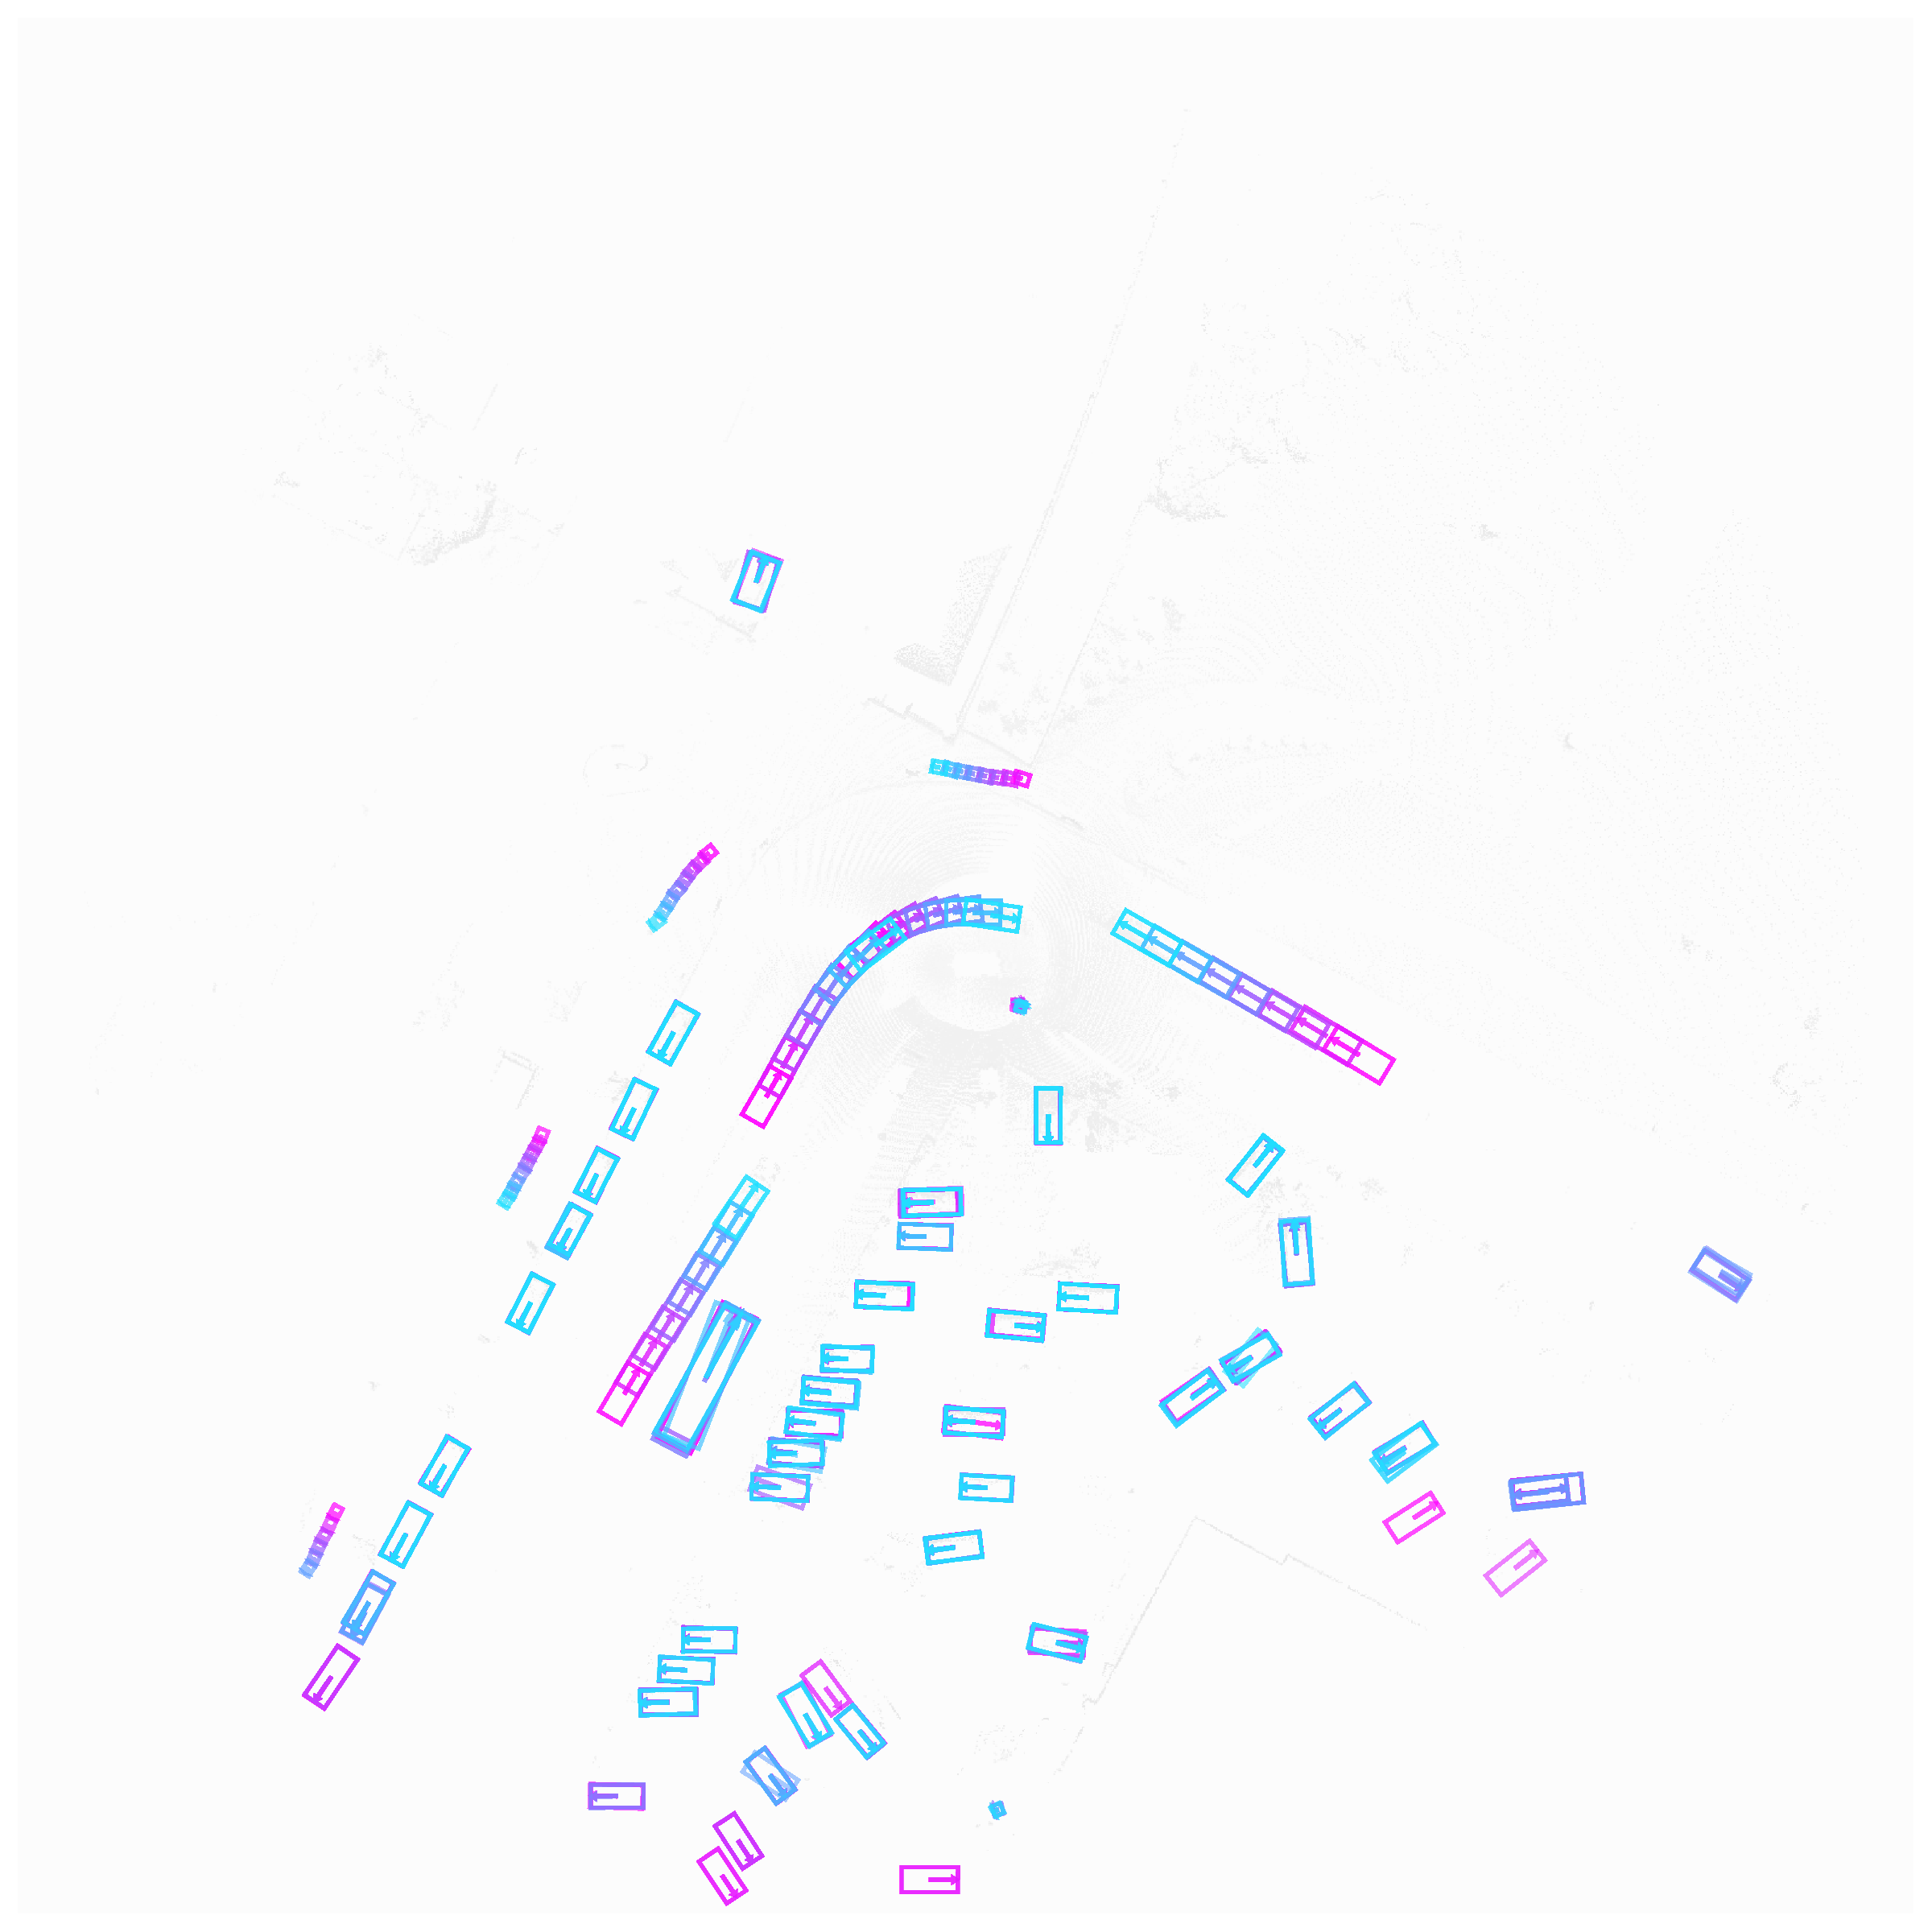
\includegraphics[width=\imw, viewport=216 7 792 583, clip]{images_for_supp/66/original_det_anchors_wod_viz_66_126.pdf}};
    \node[draw=black,very thick,anchor=west , inner sep=0pt] (S1C) at (S1B.east)  {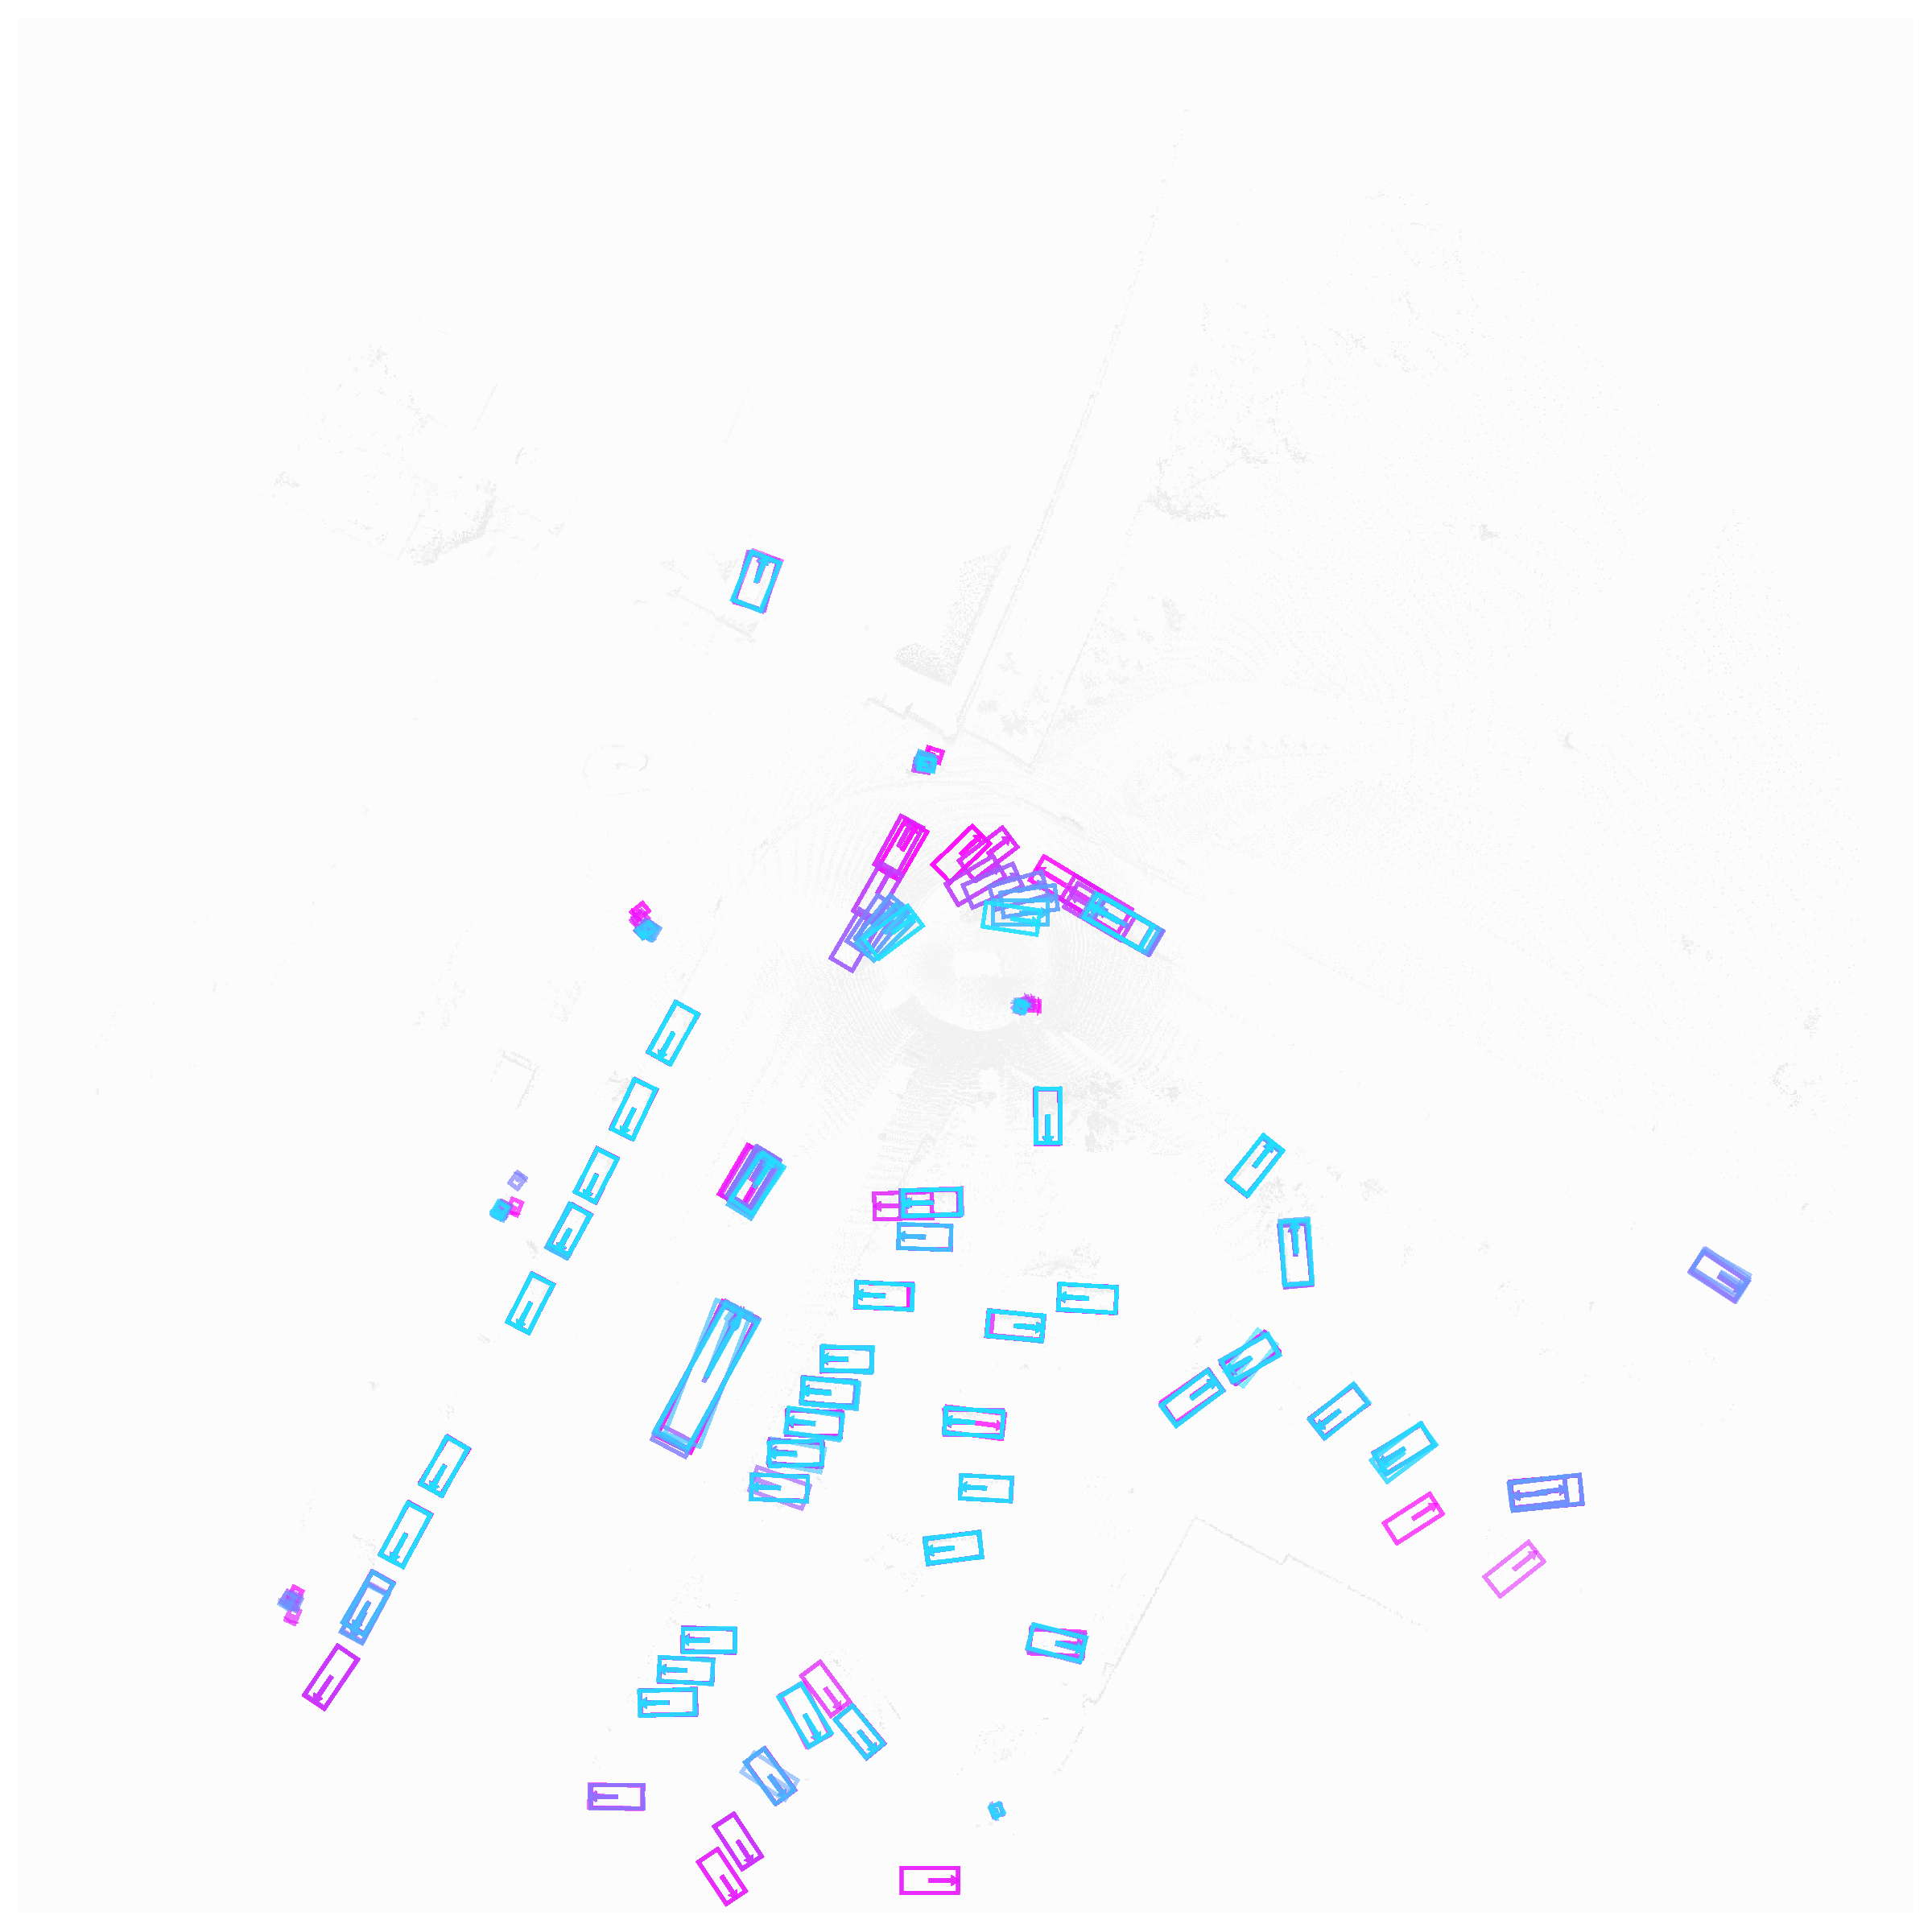
\includegraphics[width=\imw, viewport=216 7 792 583, clip]{images_for_supp/66/interpolated_det_anchors_wod_viz_66_126.pdf}};
    \node[draw=black,very thick,anchor=west, inner sep=0pt] (S1A) at (S1C.east)   {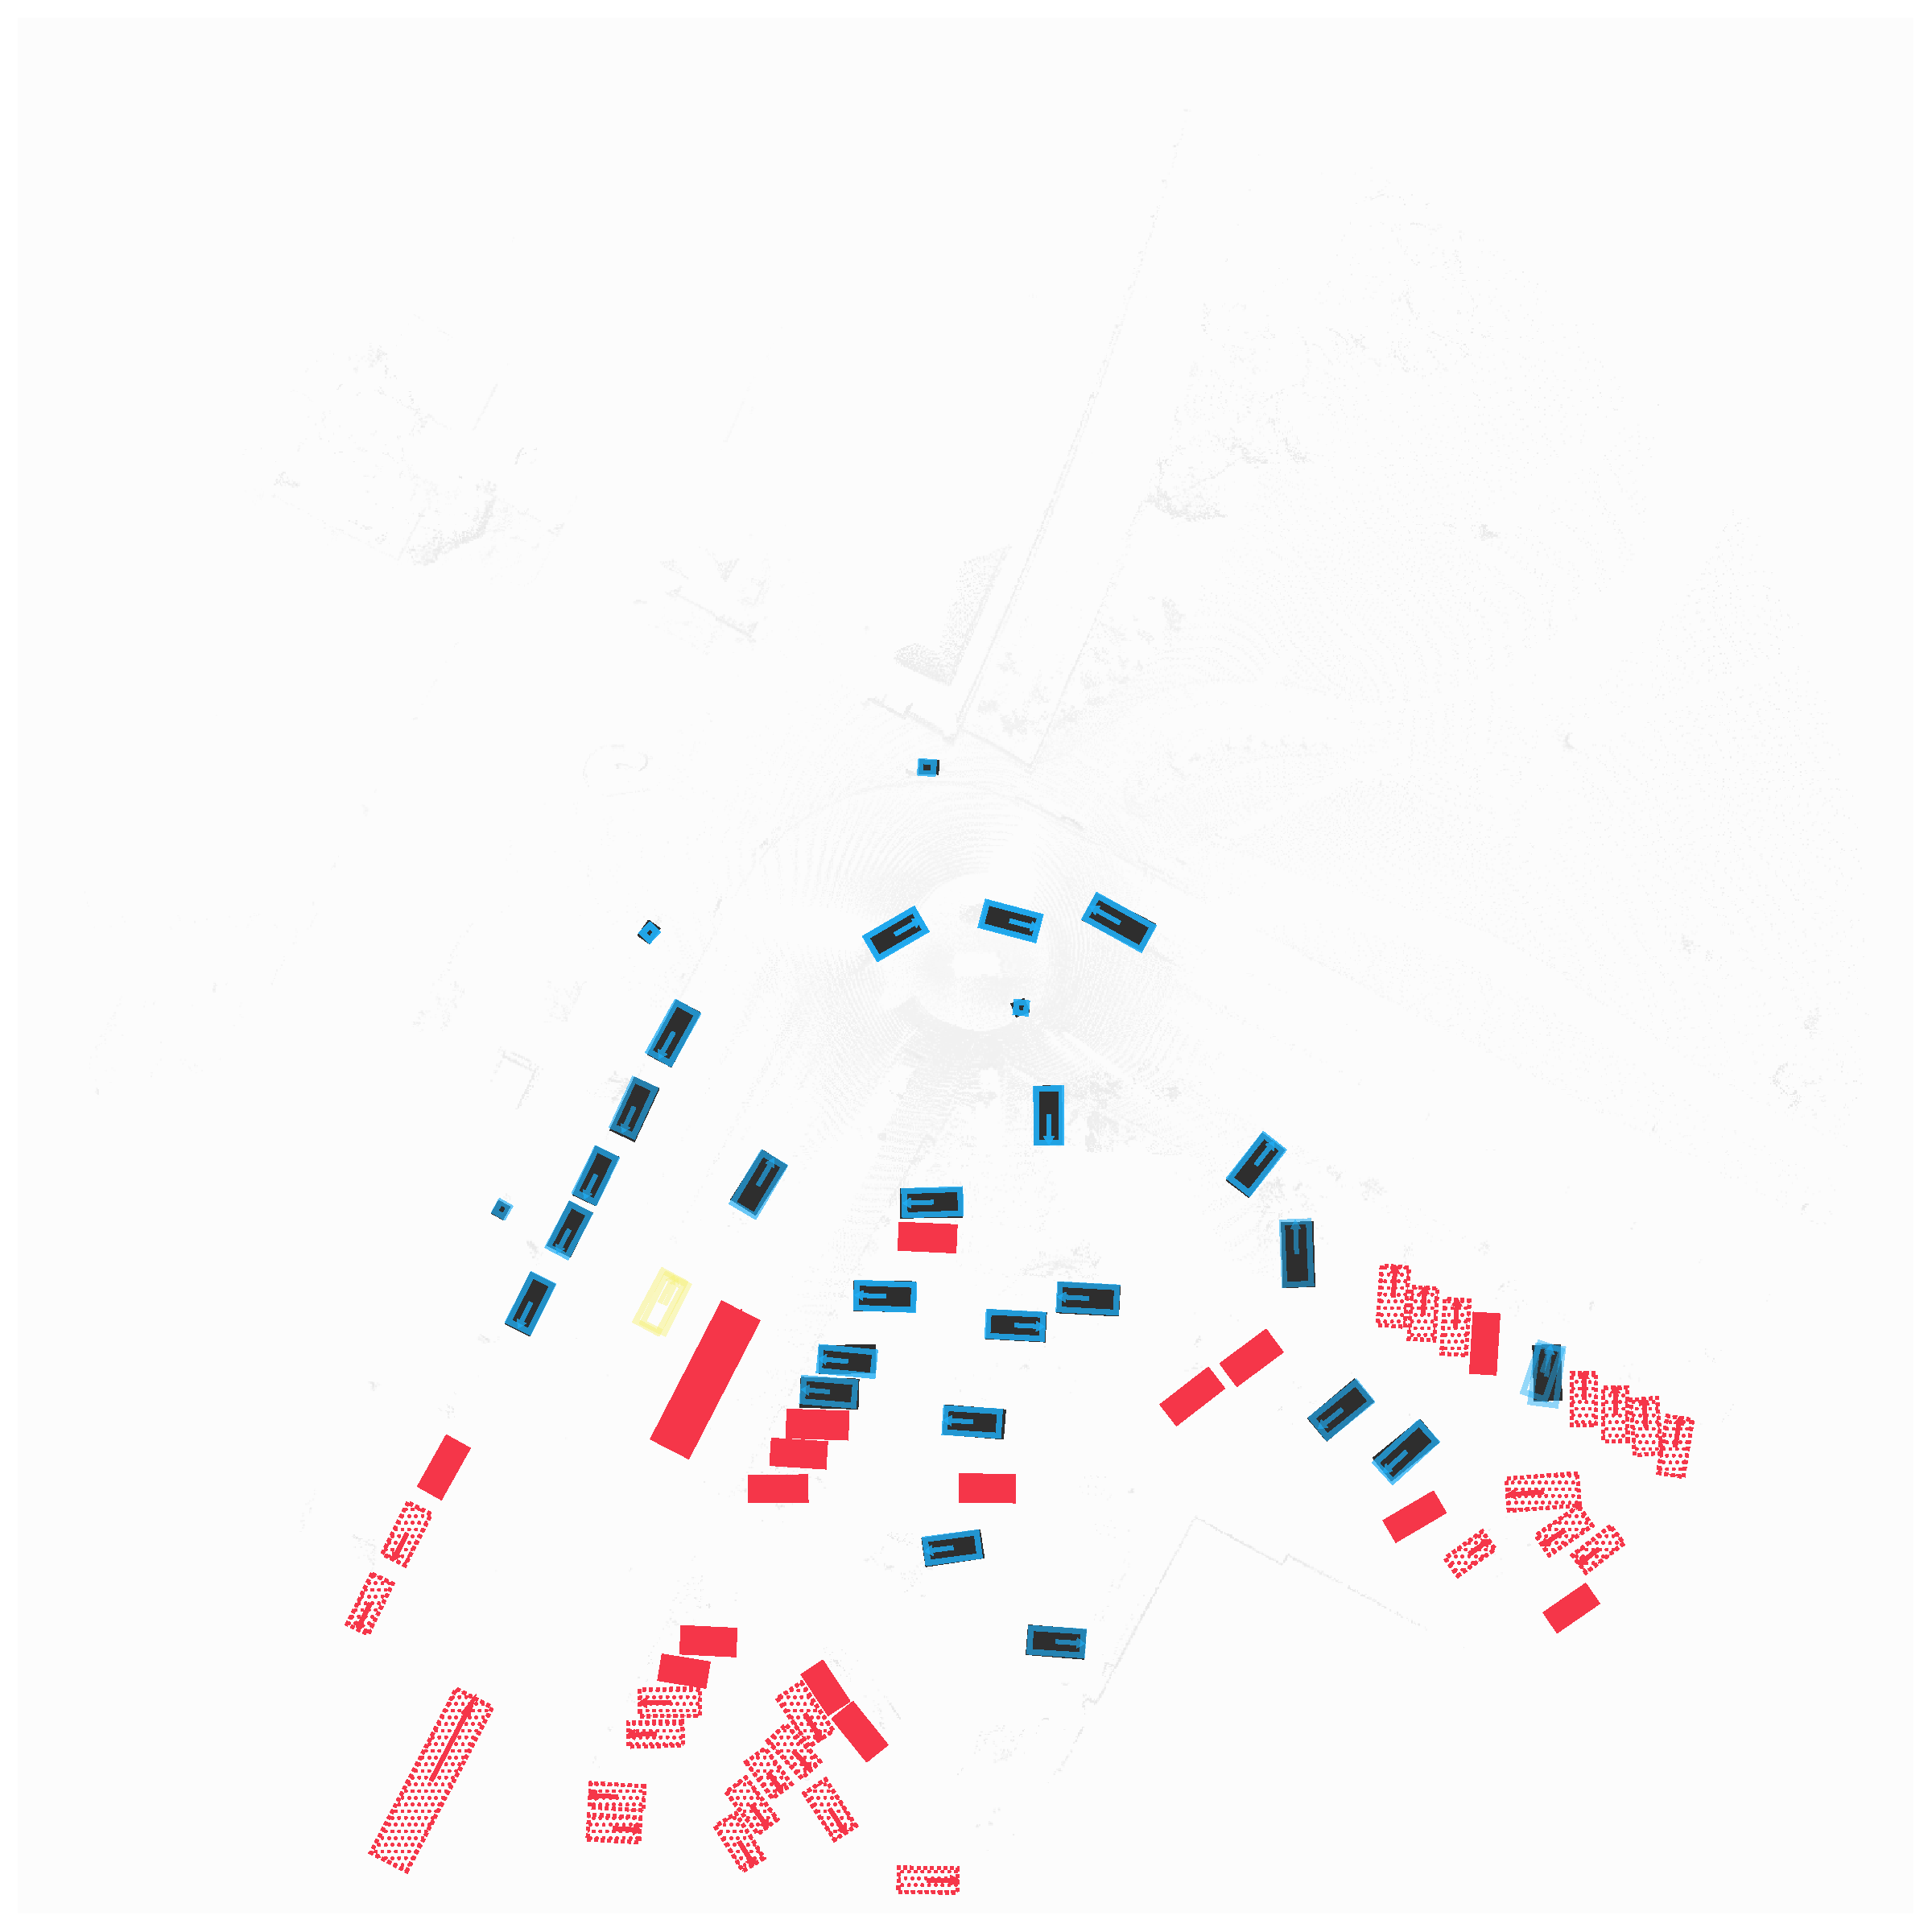
\includegraphics[width=\imw, viewport=216 7 792 583, clip]{images_for_supp/66/lidar_proposals_wod_viz_66_126.pdf}};
    \node[draw=black,very thick,anchor=west , inner sep=0pt] (S1D) at (S1A.east)  {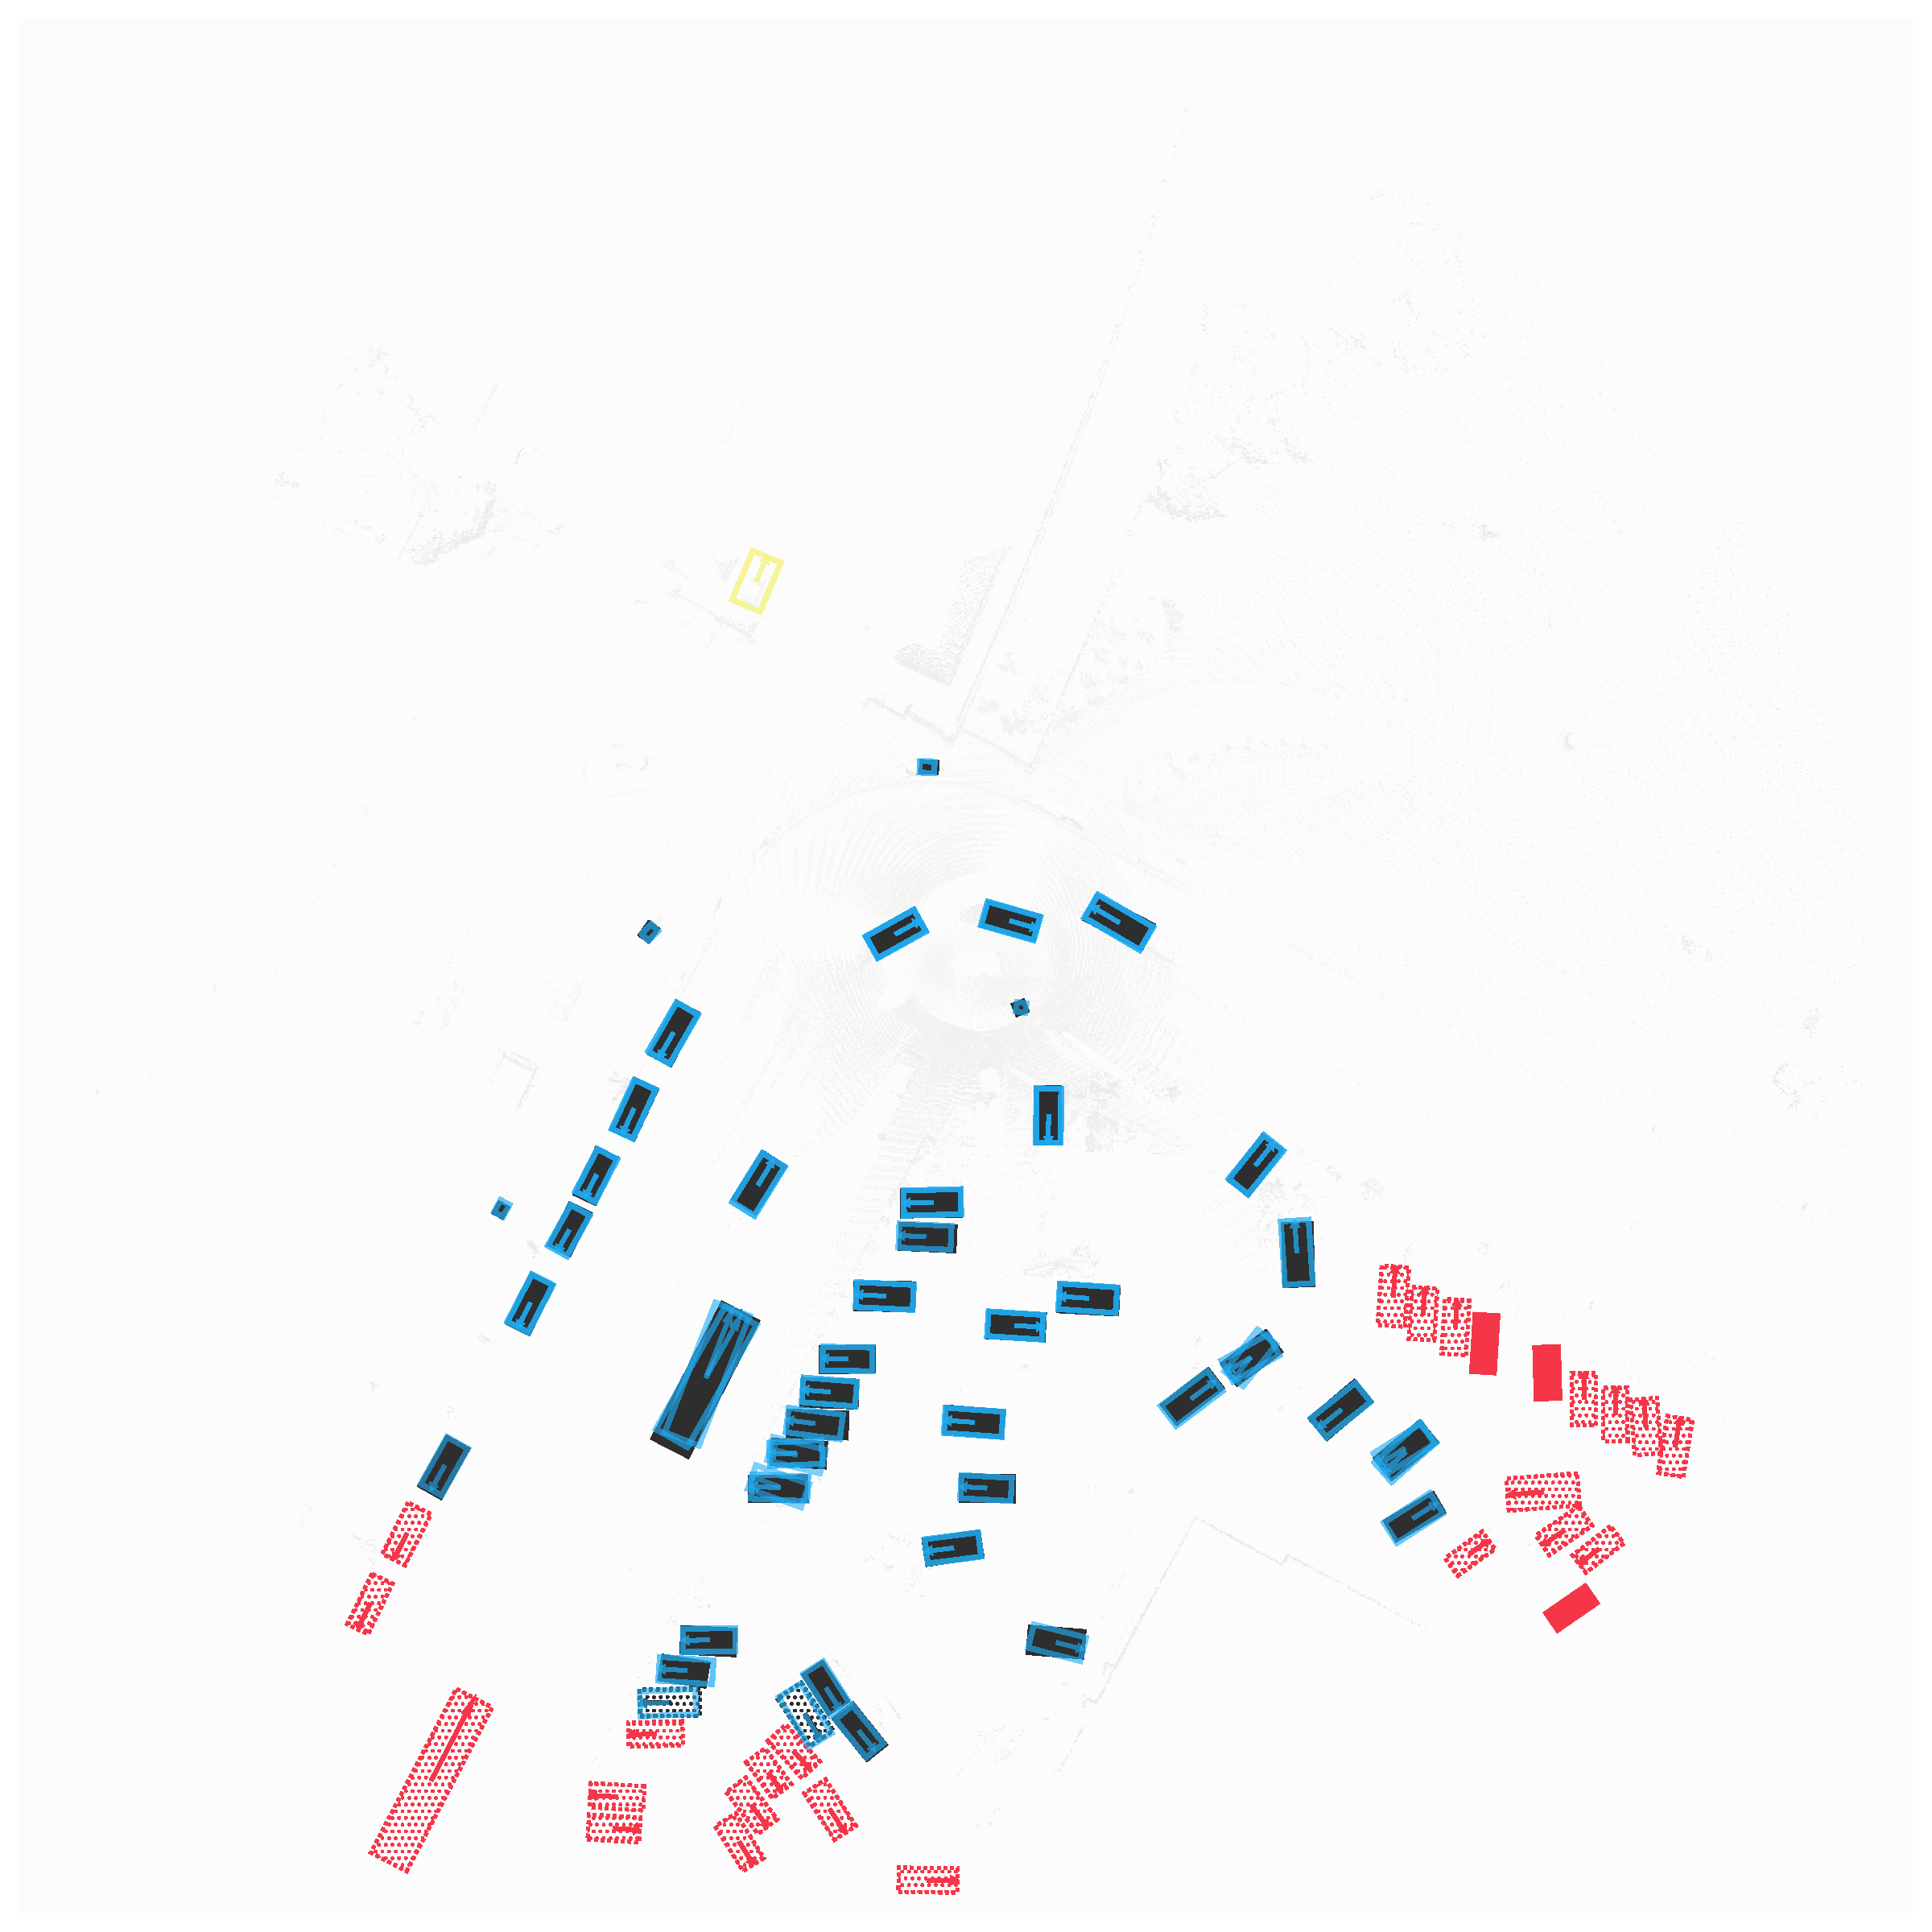
\includegraphics[width=\imw, viewport=216 7 792 583, clip]{images_for_supp/66/detections_wod_viz_66_126.pdf}};

    % \node at (S1A.north) [anchor=south] {\small Detection Proposal Boxes $\mathbf{B}^\mathrm{det}$};
    % \node at (S1B.north) [anchor=south] {\small Memory Bank};
    % \node at (S1C.north) [anchor=south] {\small Memory Proposal Boxes $\mathbf{B}^\mathrm{mem}$};
    % \node at (S1D.north) [anchor=south] {\small \ourmodel{} Output Boxes $\mathbf{B}^\mathrm{ref}$};

    \node[draw=black,very thick,anchor=north, inner sep=0pt] (S2A) at ([yshift=-\rowsep]S1B.south) {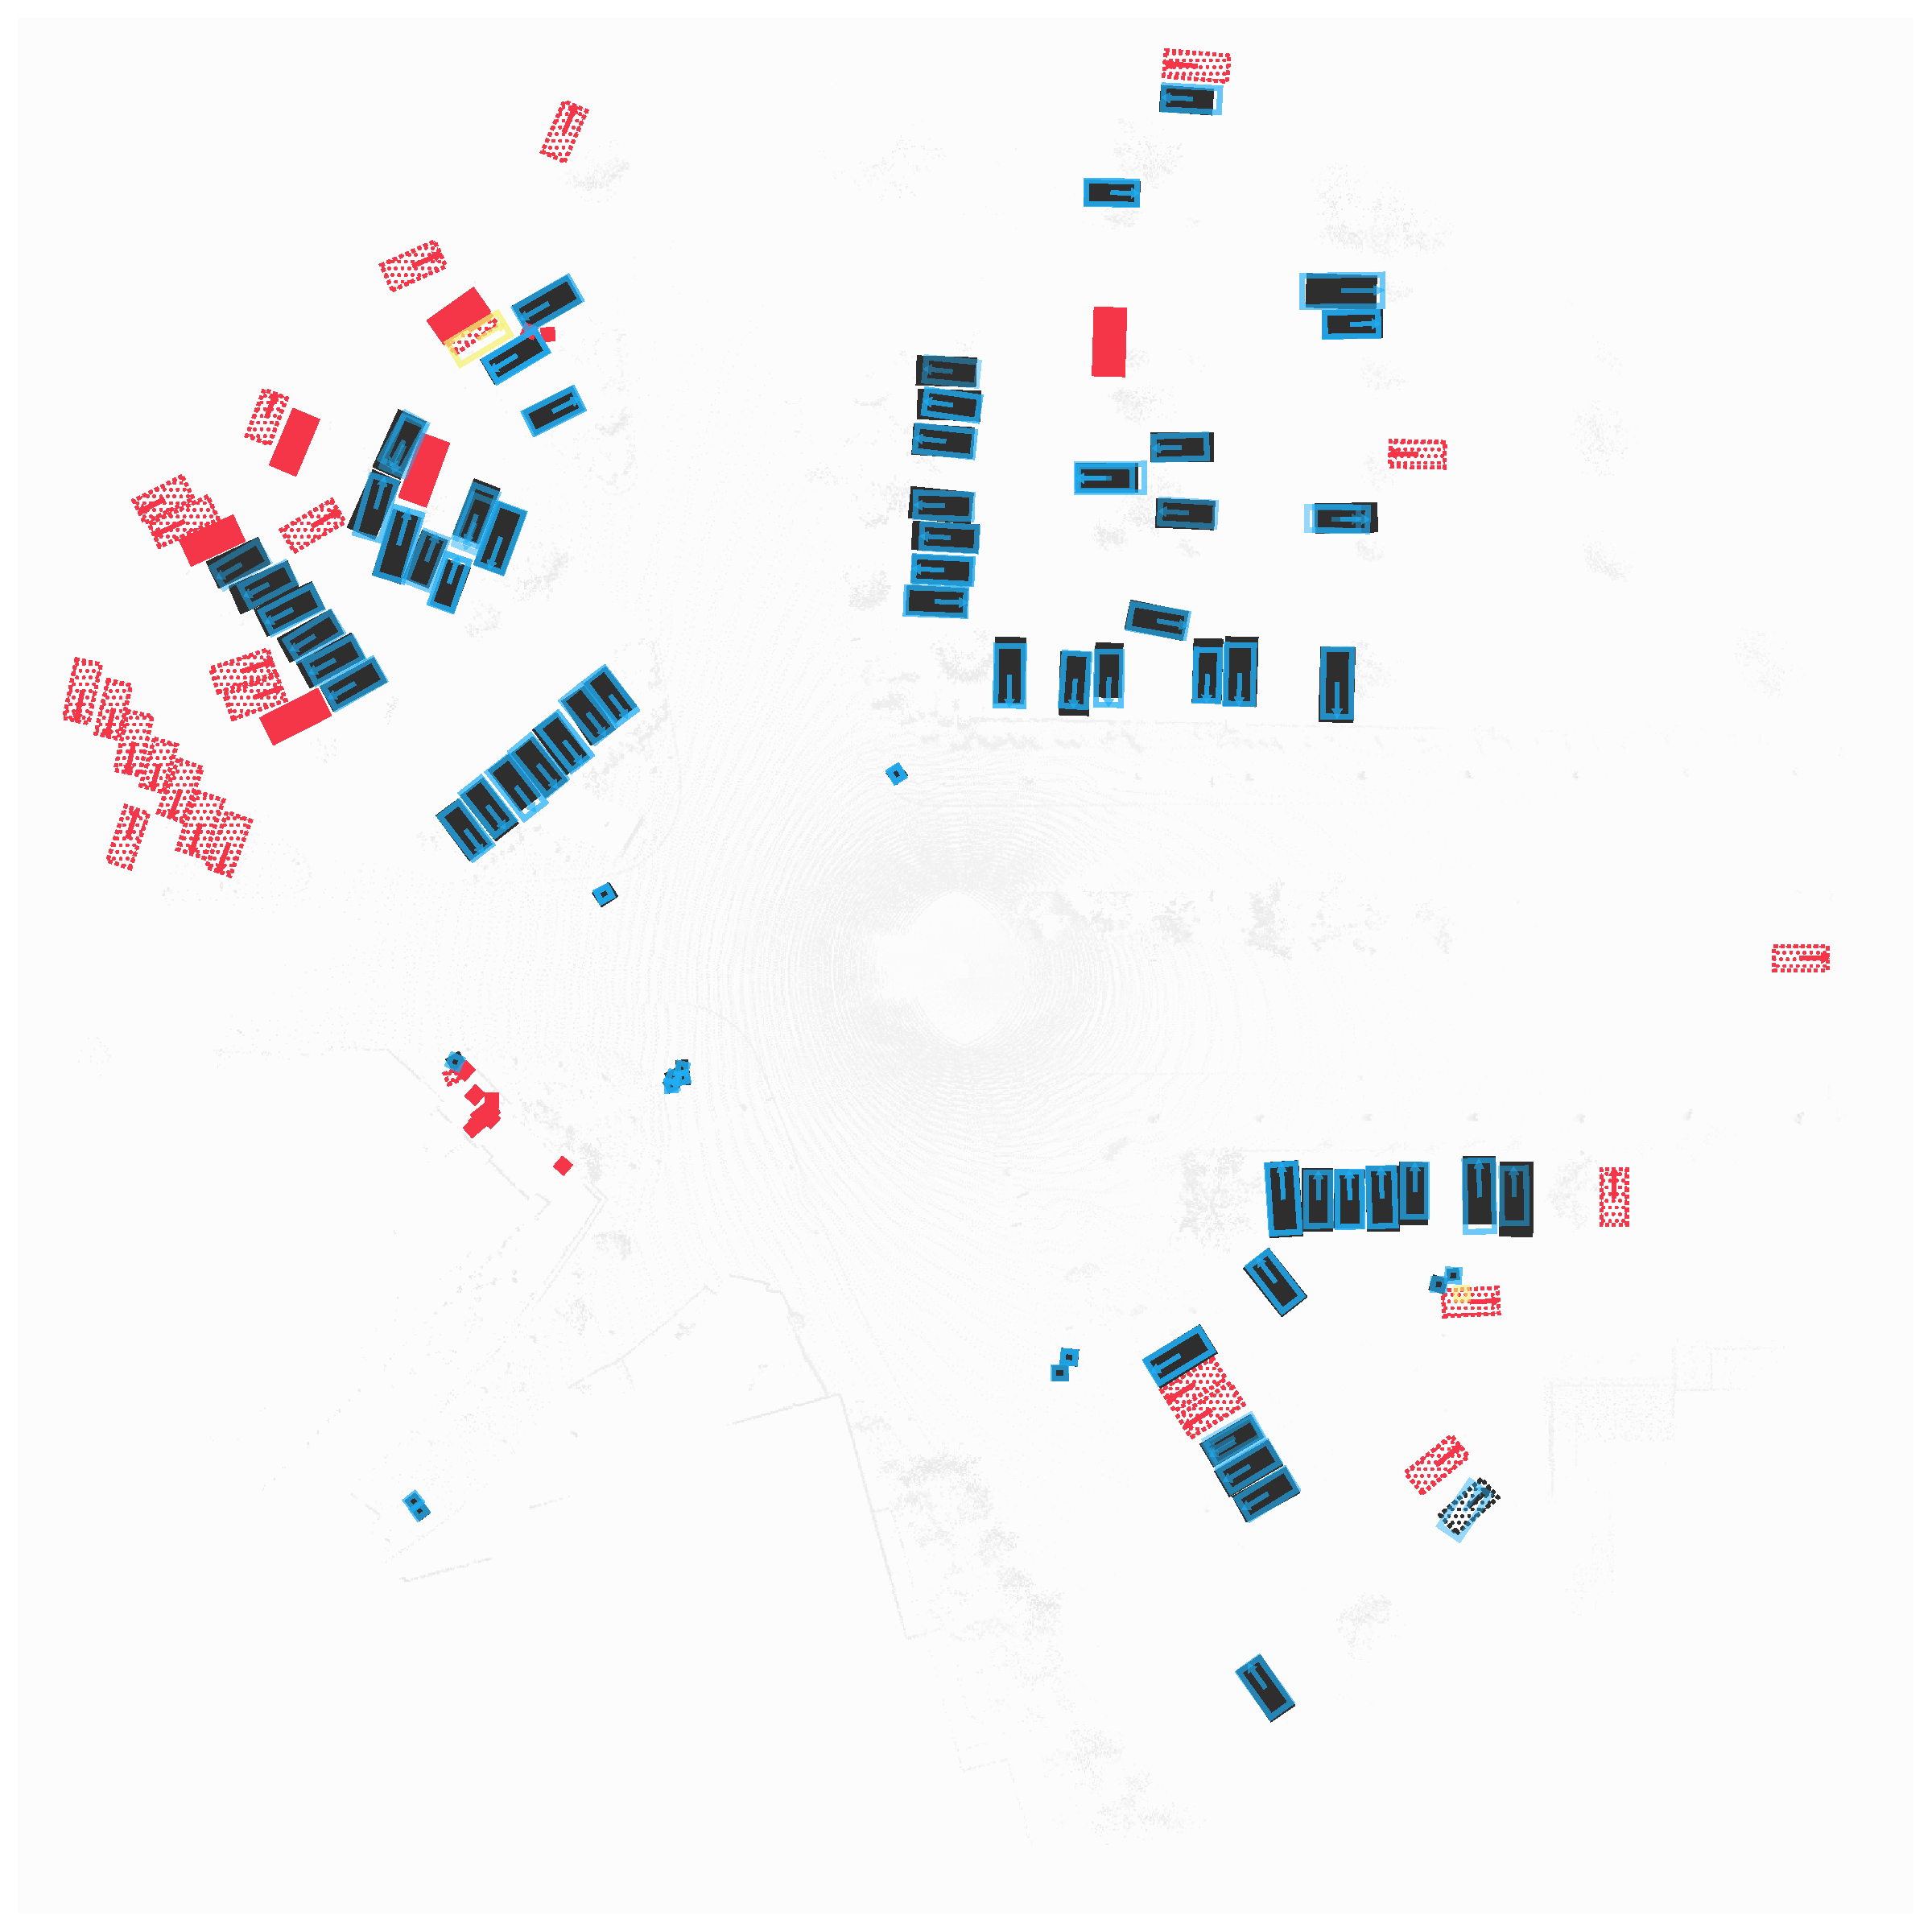
\includegraphics[width=\imw, viewport=14 432 518 936, clip]{images_for_supp/98/lidar_proposals_wod_viz_98_138.pdf}};
    \node[draw=black,very thick,anchor=west, inner sep=0pt]  (S2B) at (S2A.east)                   {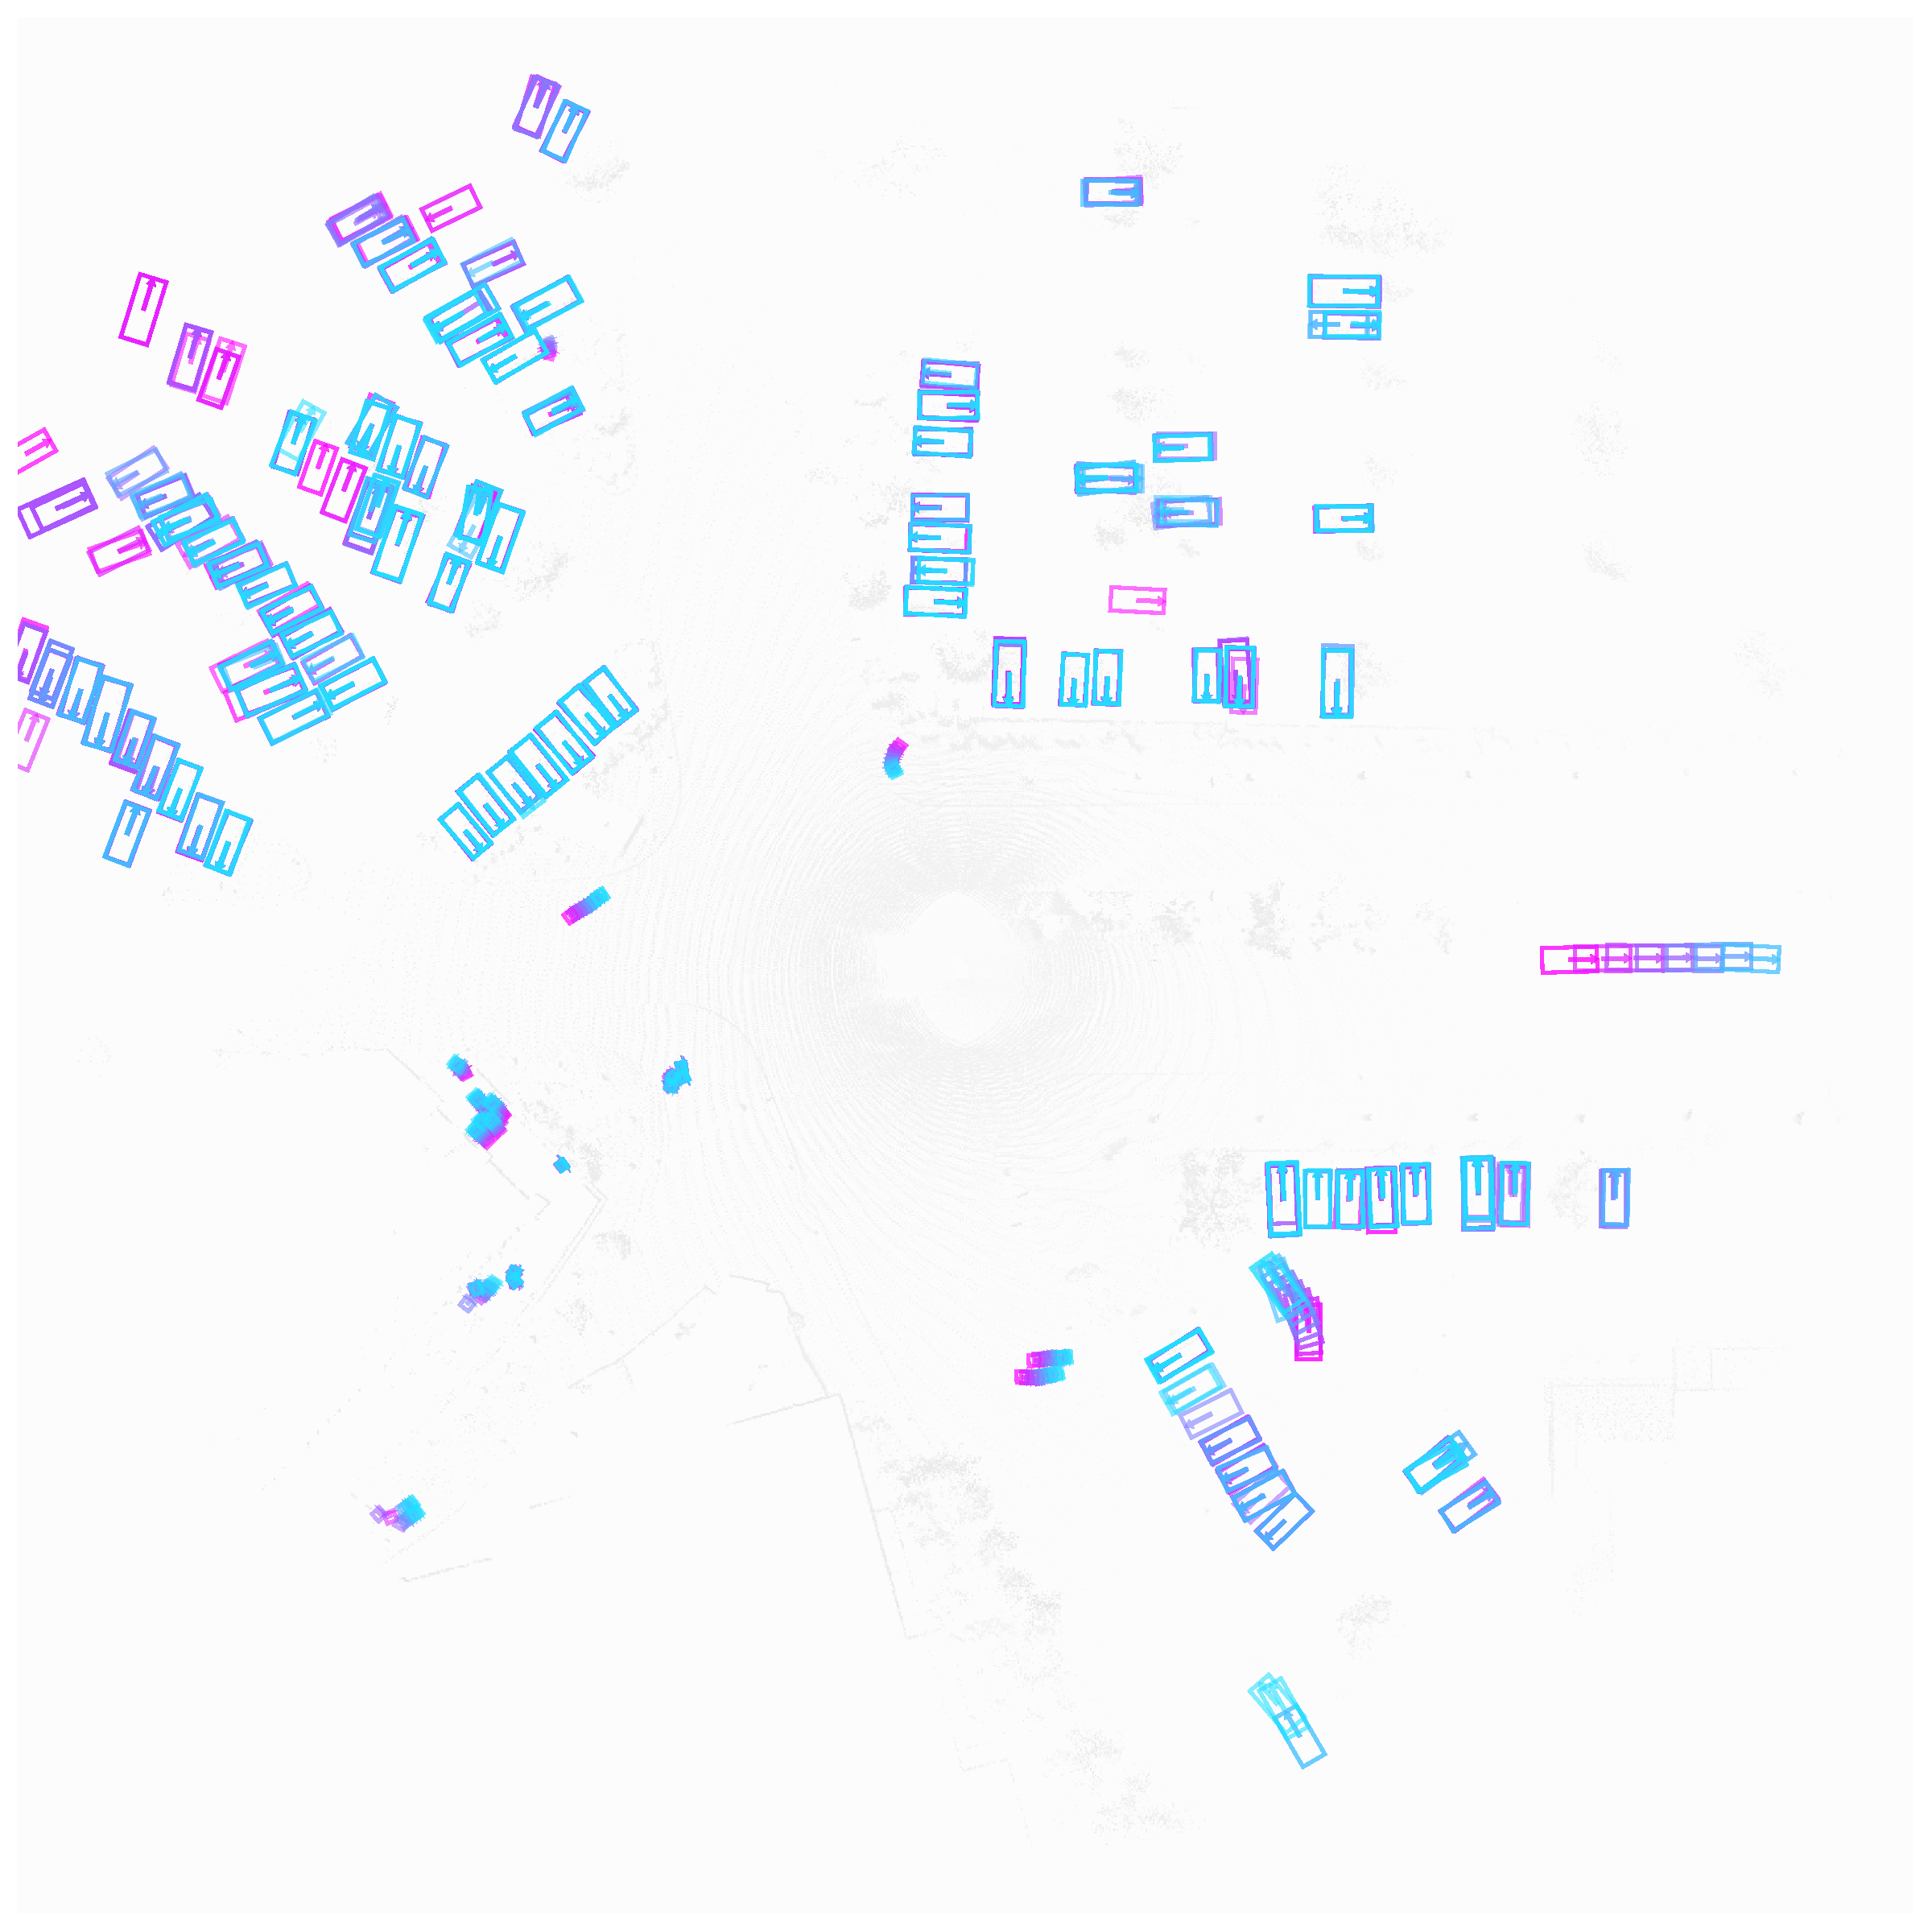
\includegraphics[width=\imw, viewport=14 432 518 936, clip]{images_for_supp/98/original_det_anchors_wod_viz_98_138.pdf}};
    \node[draw=black,very thick,anchor=west, inner sep=0pt]  (S2C) at (S2B.east)                   {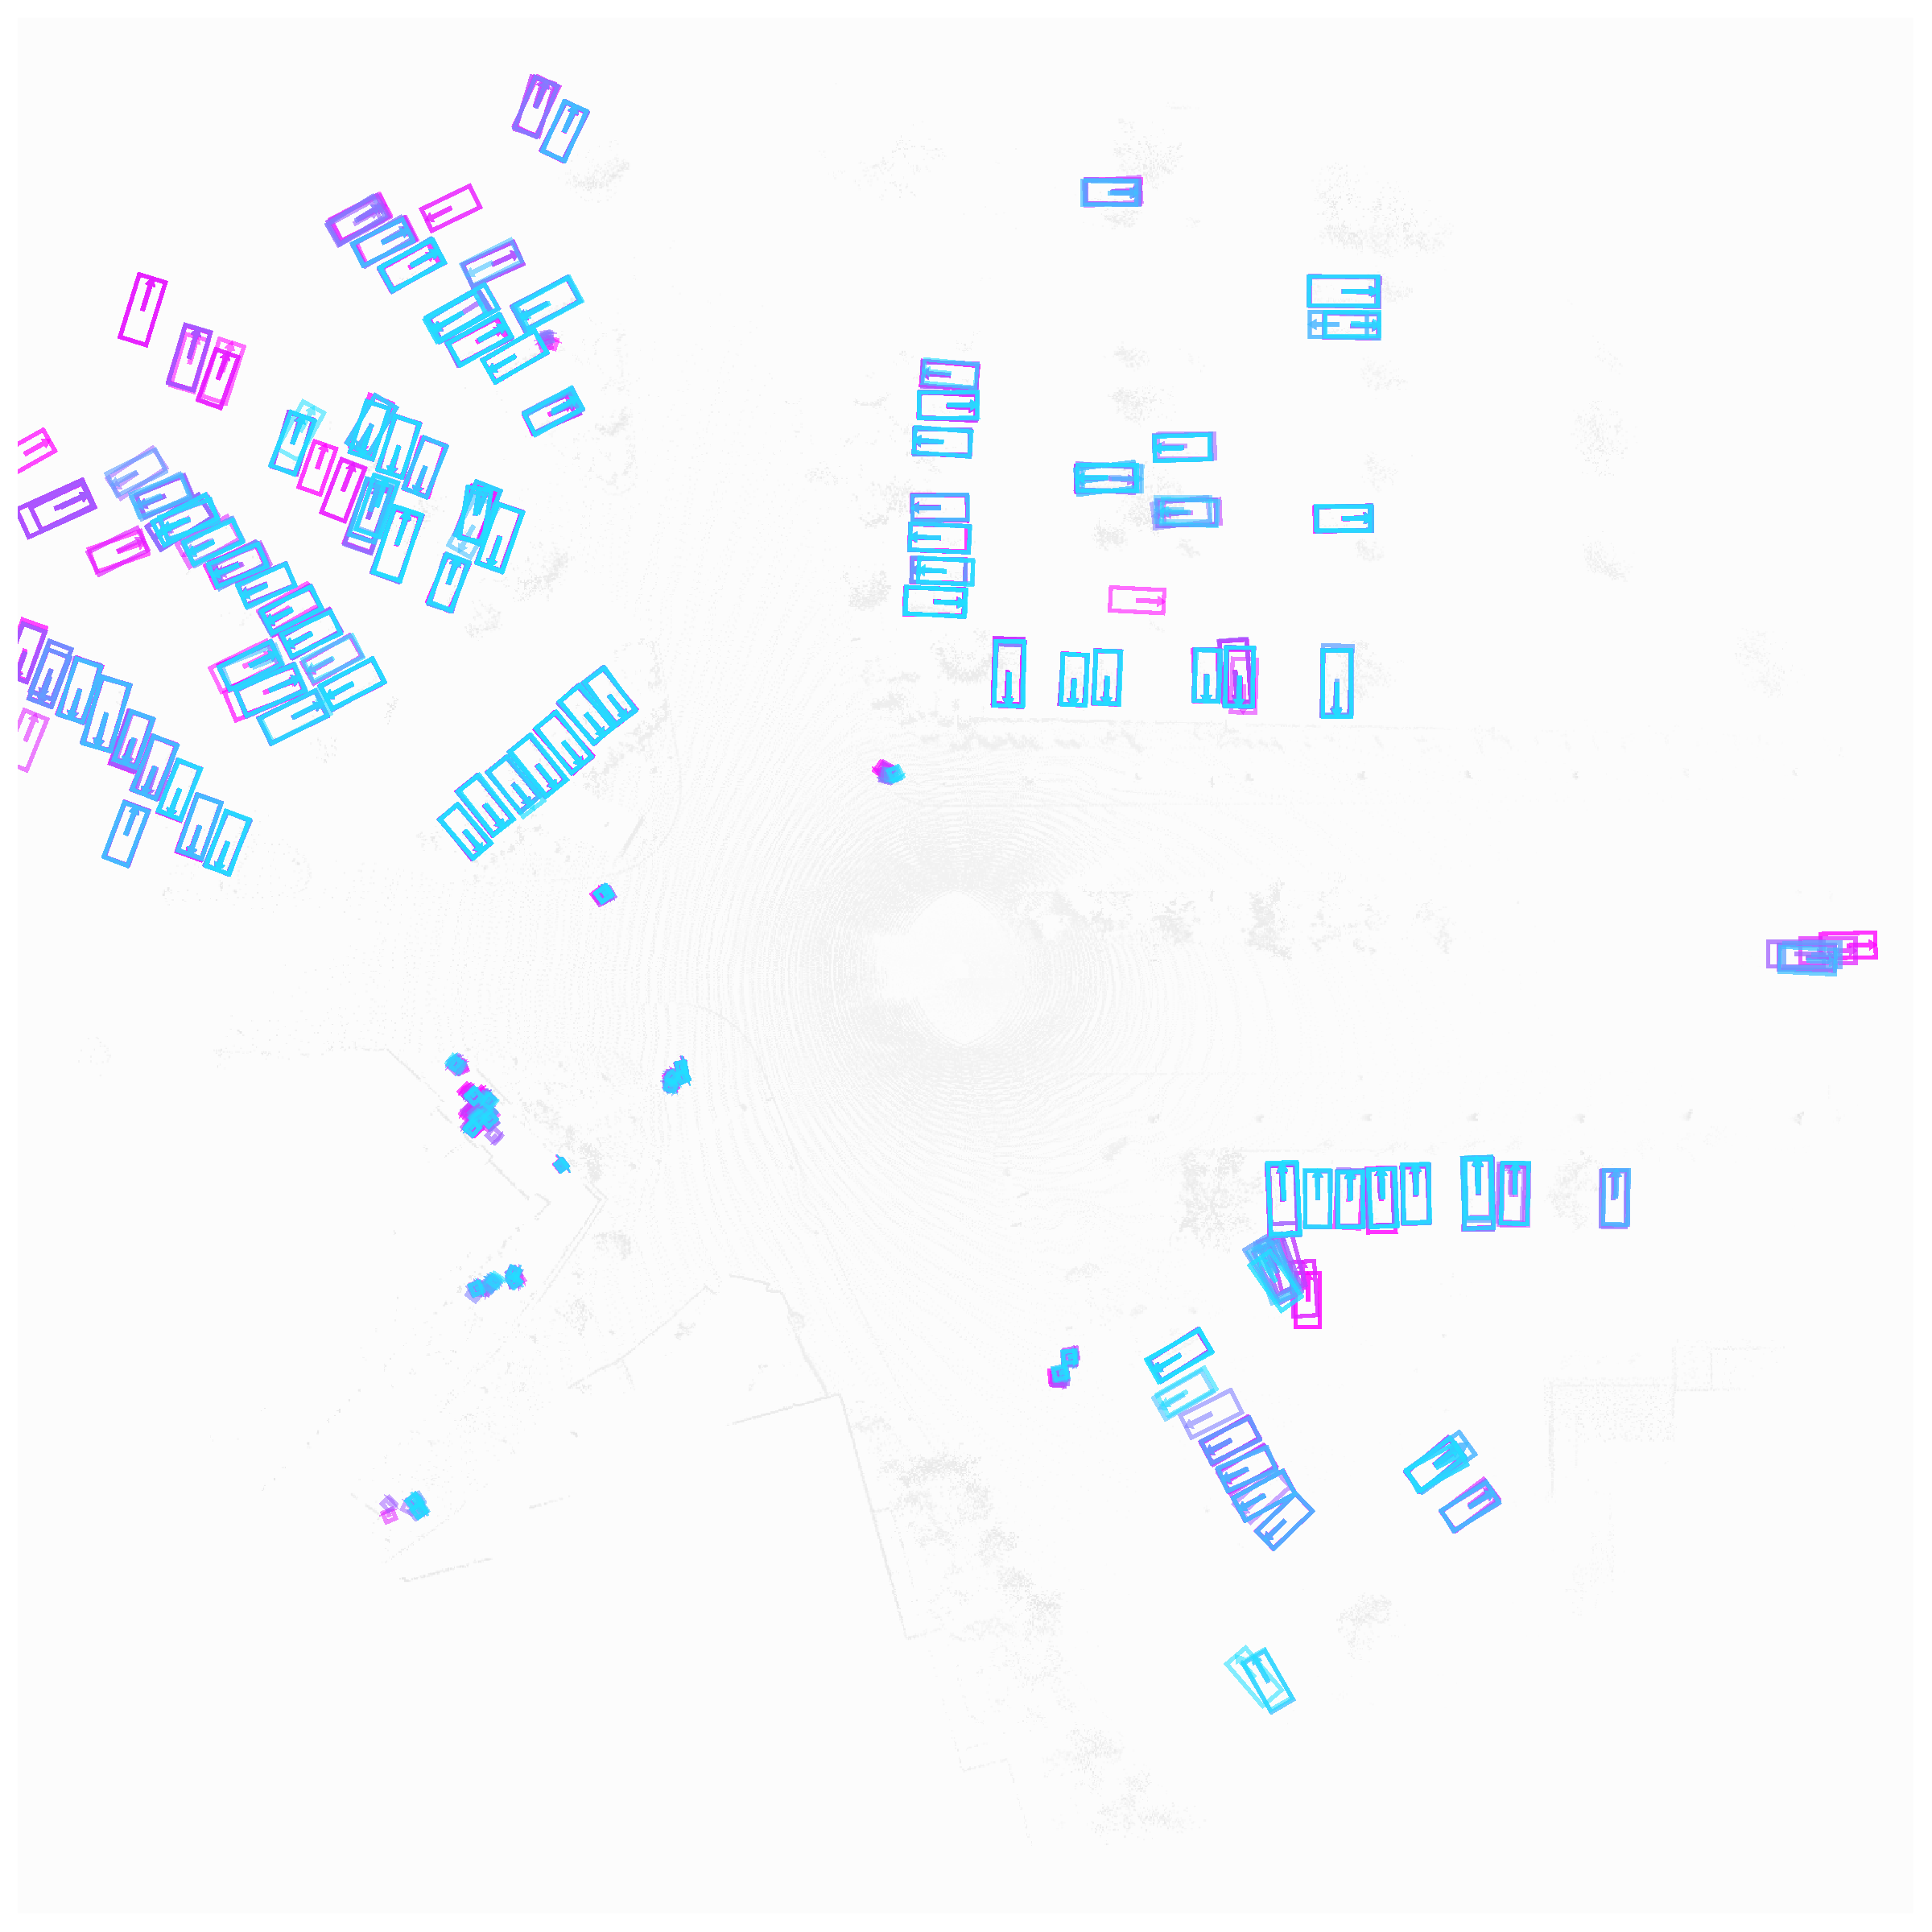
\includegraphics[width=\imw, viewport=14 432 518 936, clip]{images_for_supp/98/interpolated_det_anchors_wod_viz_98_138.pdf}};
    \node[draw=black,very thick,anchor=west, inner sep=0pt]  (S2D) at (S2C.east)                   {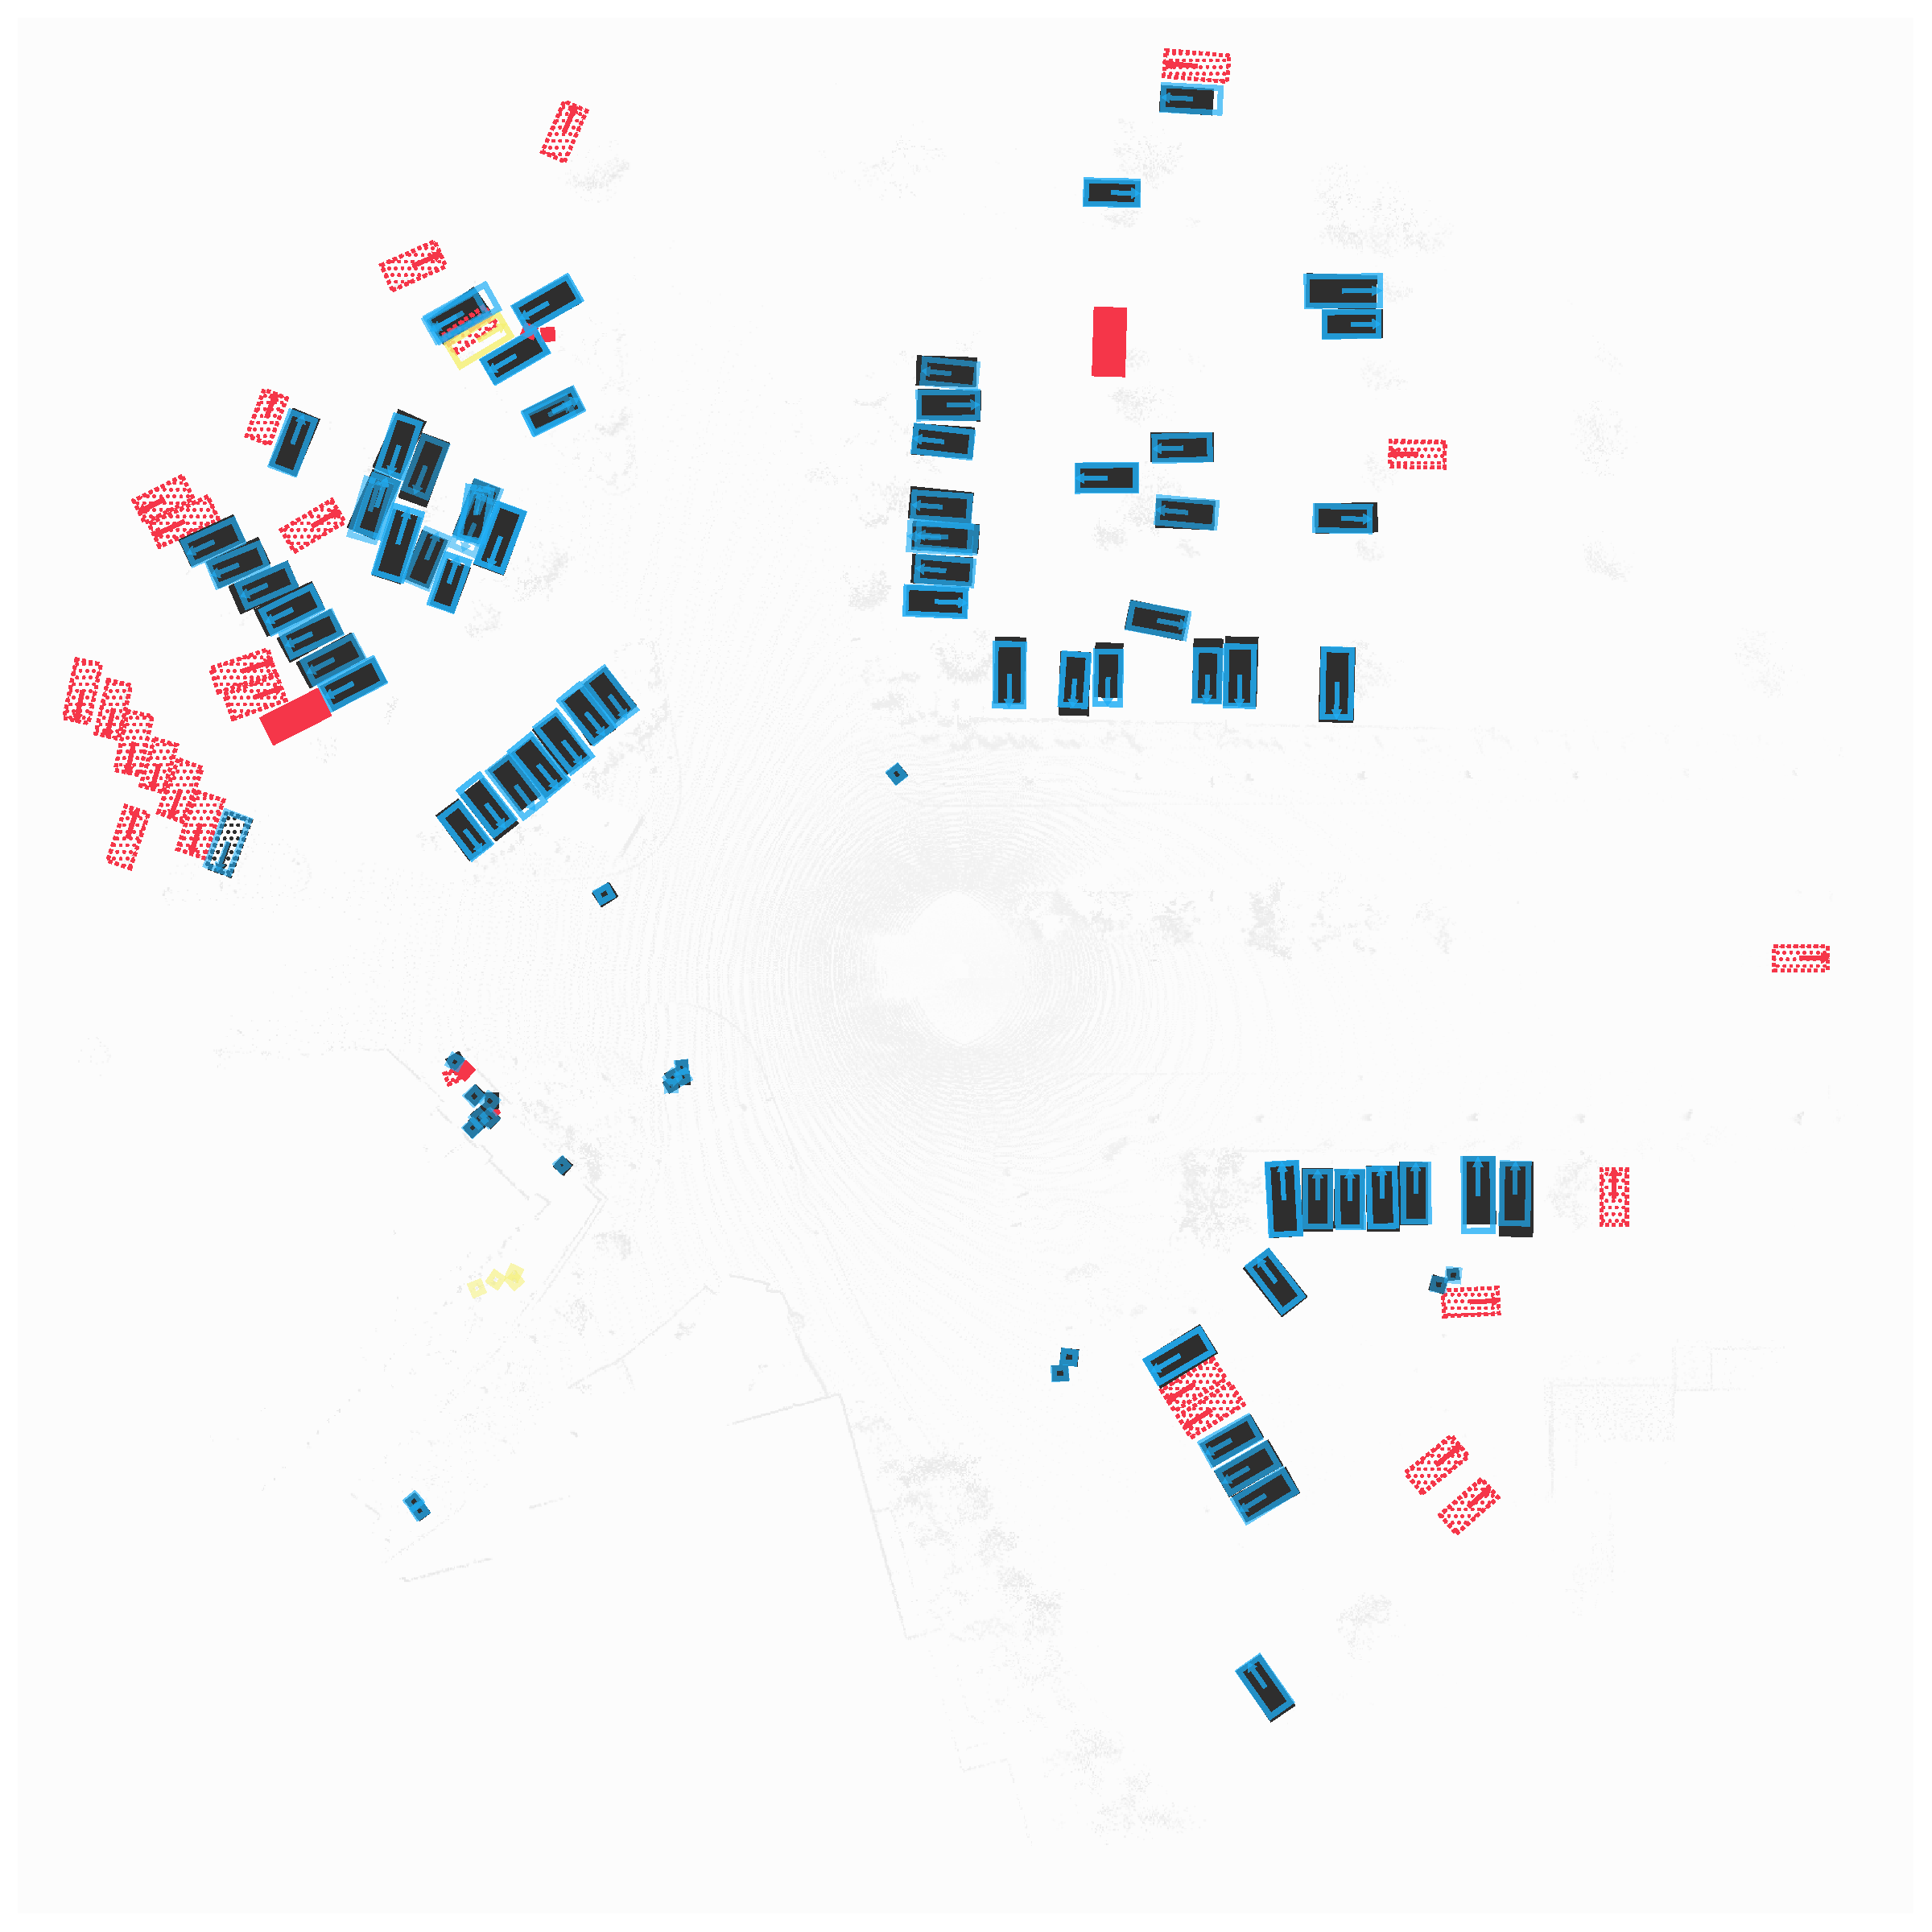
\includegraphics[width=\imw, viewport=14 432 518 936, clip]{images_for_supp/98/detections_wod_viz_98_138.pdf}};

                                                                                                                            % 72 288 936 1152
    \node[draw=black,very thick,anchor=north,inner sep=0pt] (S3A) at ([yshift=-\rowsep]S2A.south) {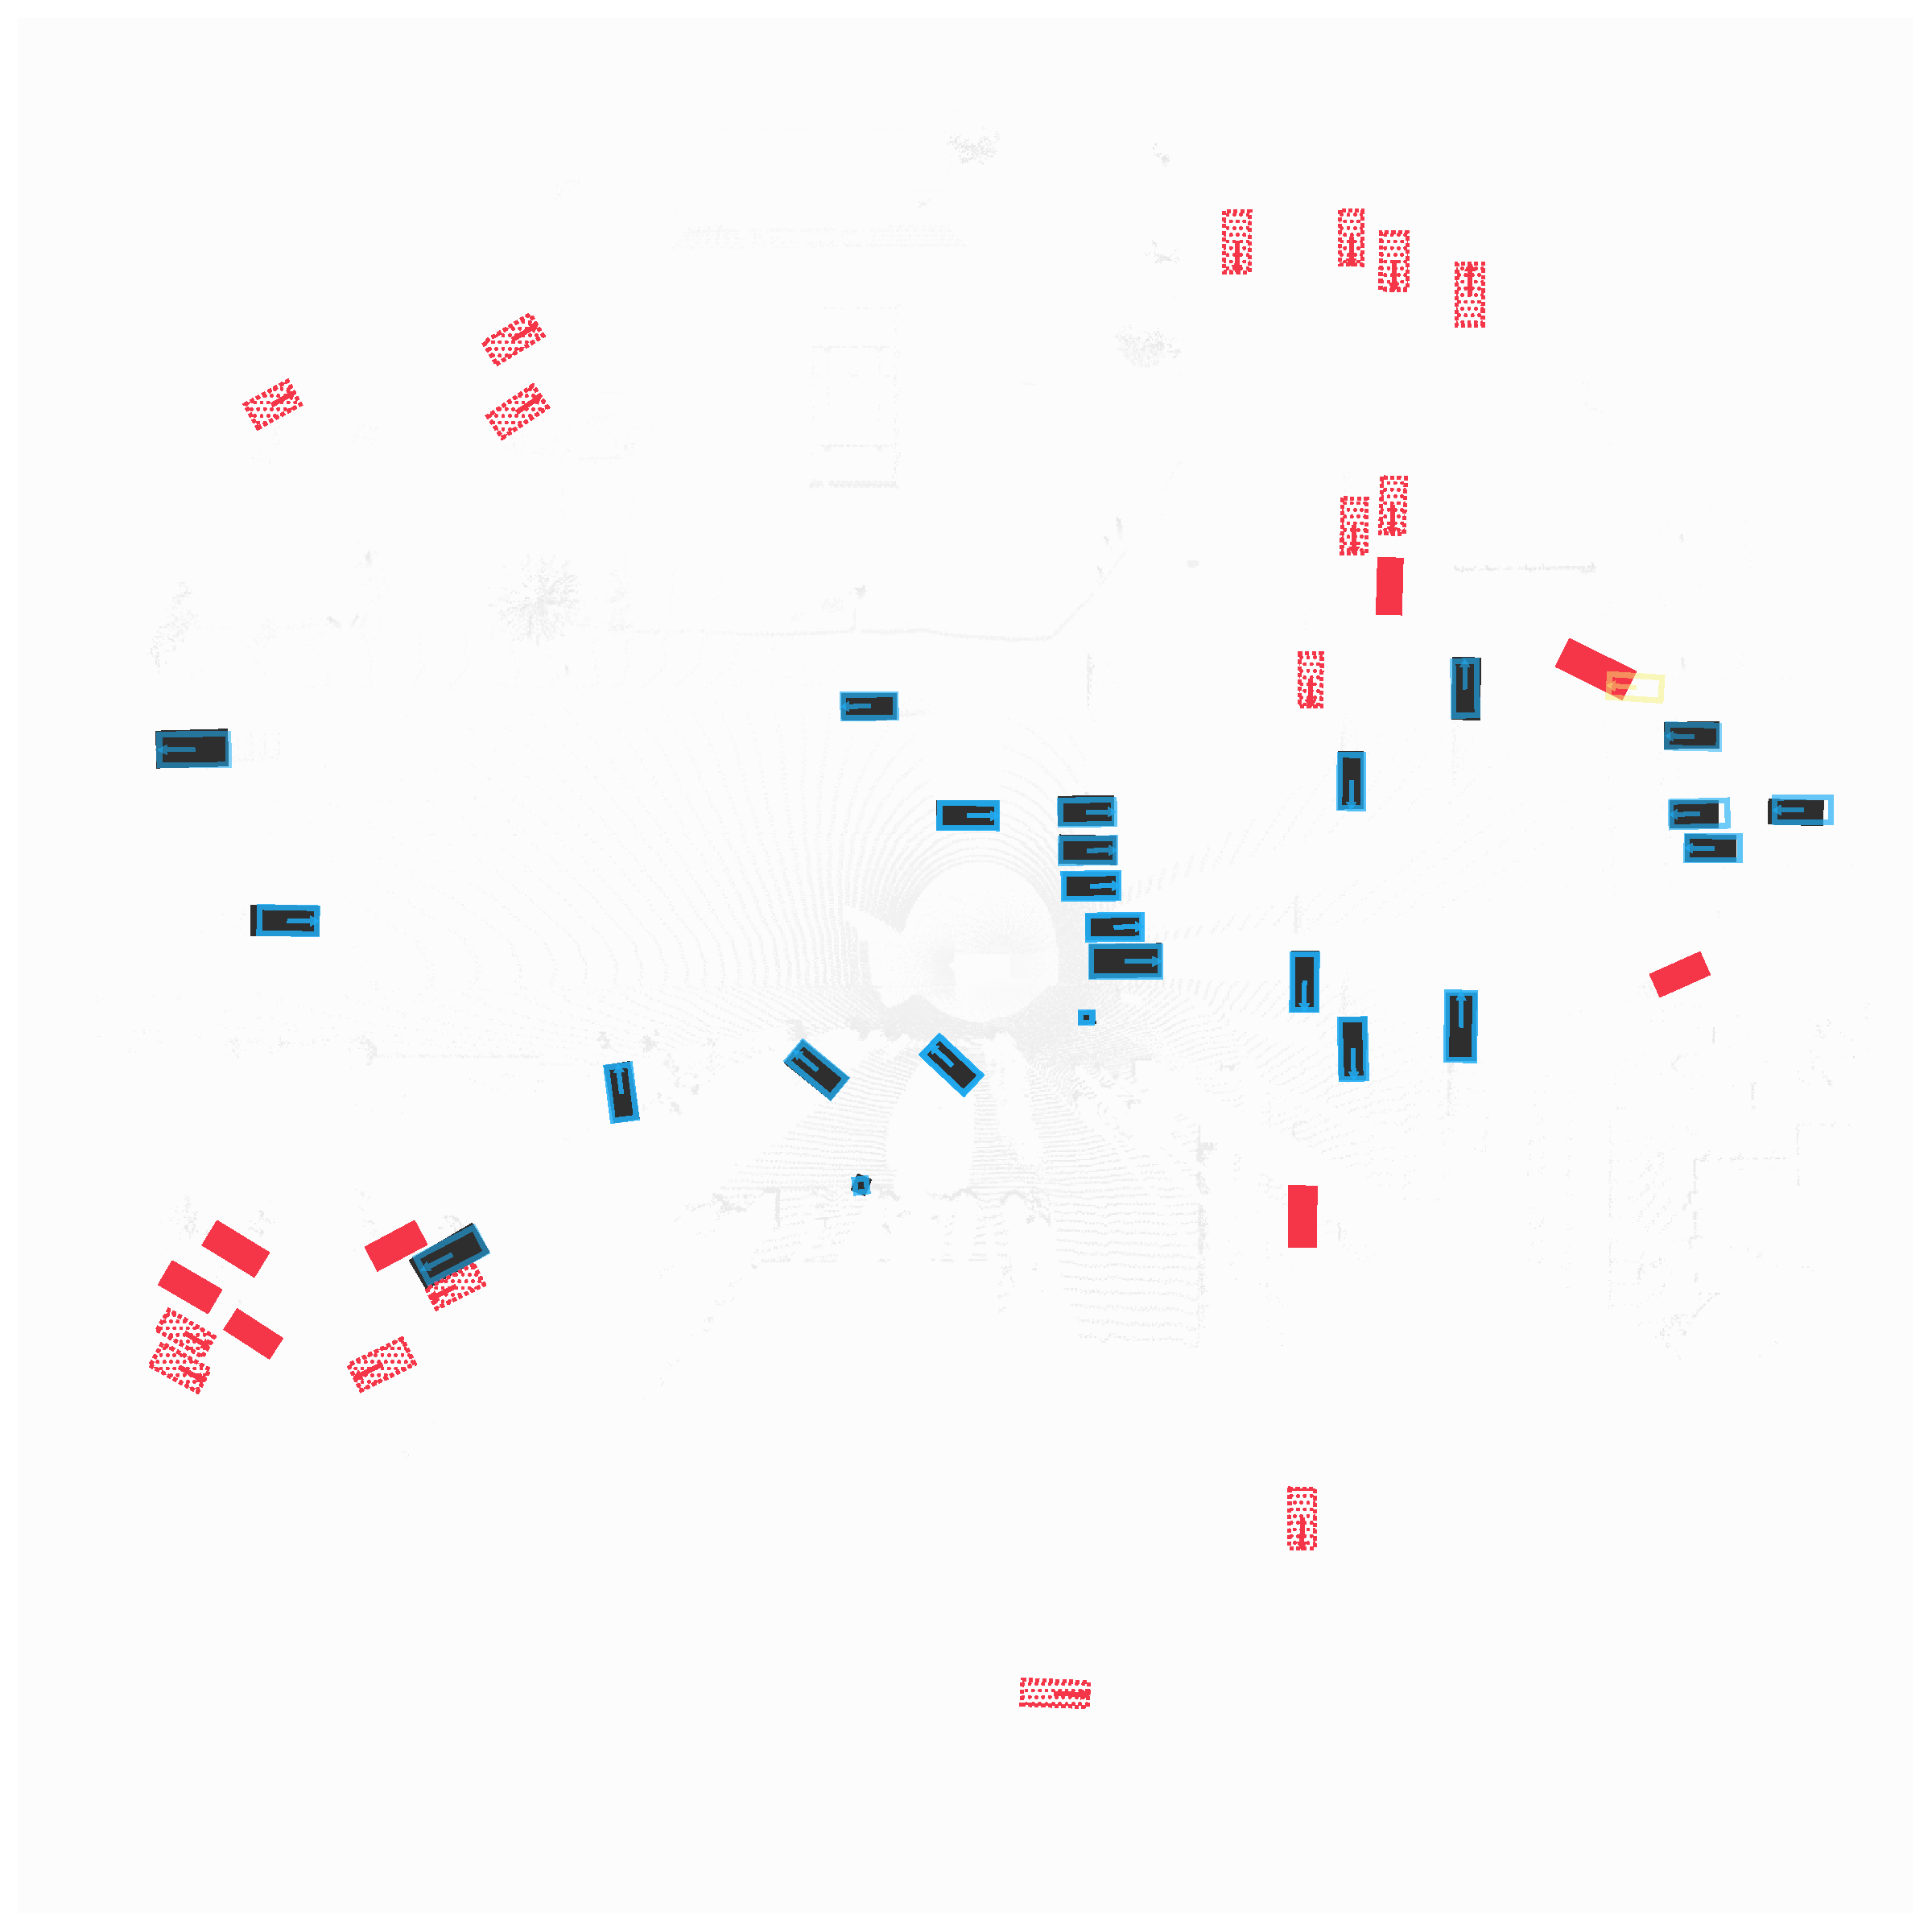
\includegraphics[width=\imw, viewport=72 288 936 1152, clip]{images_for_supp/64/lidar_proposals_wod_viz_64_90.pdf}};
    \node[draw=black,very thick,anchor=west ,inner sep=0pt]  (S3B) at (S3A.east)                   {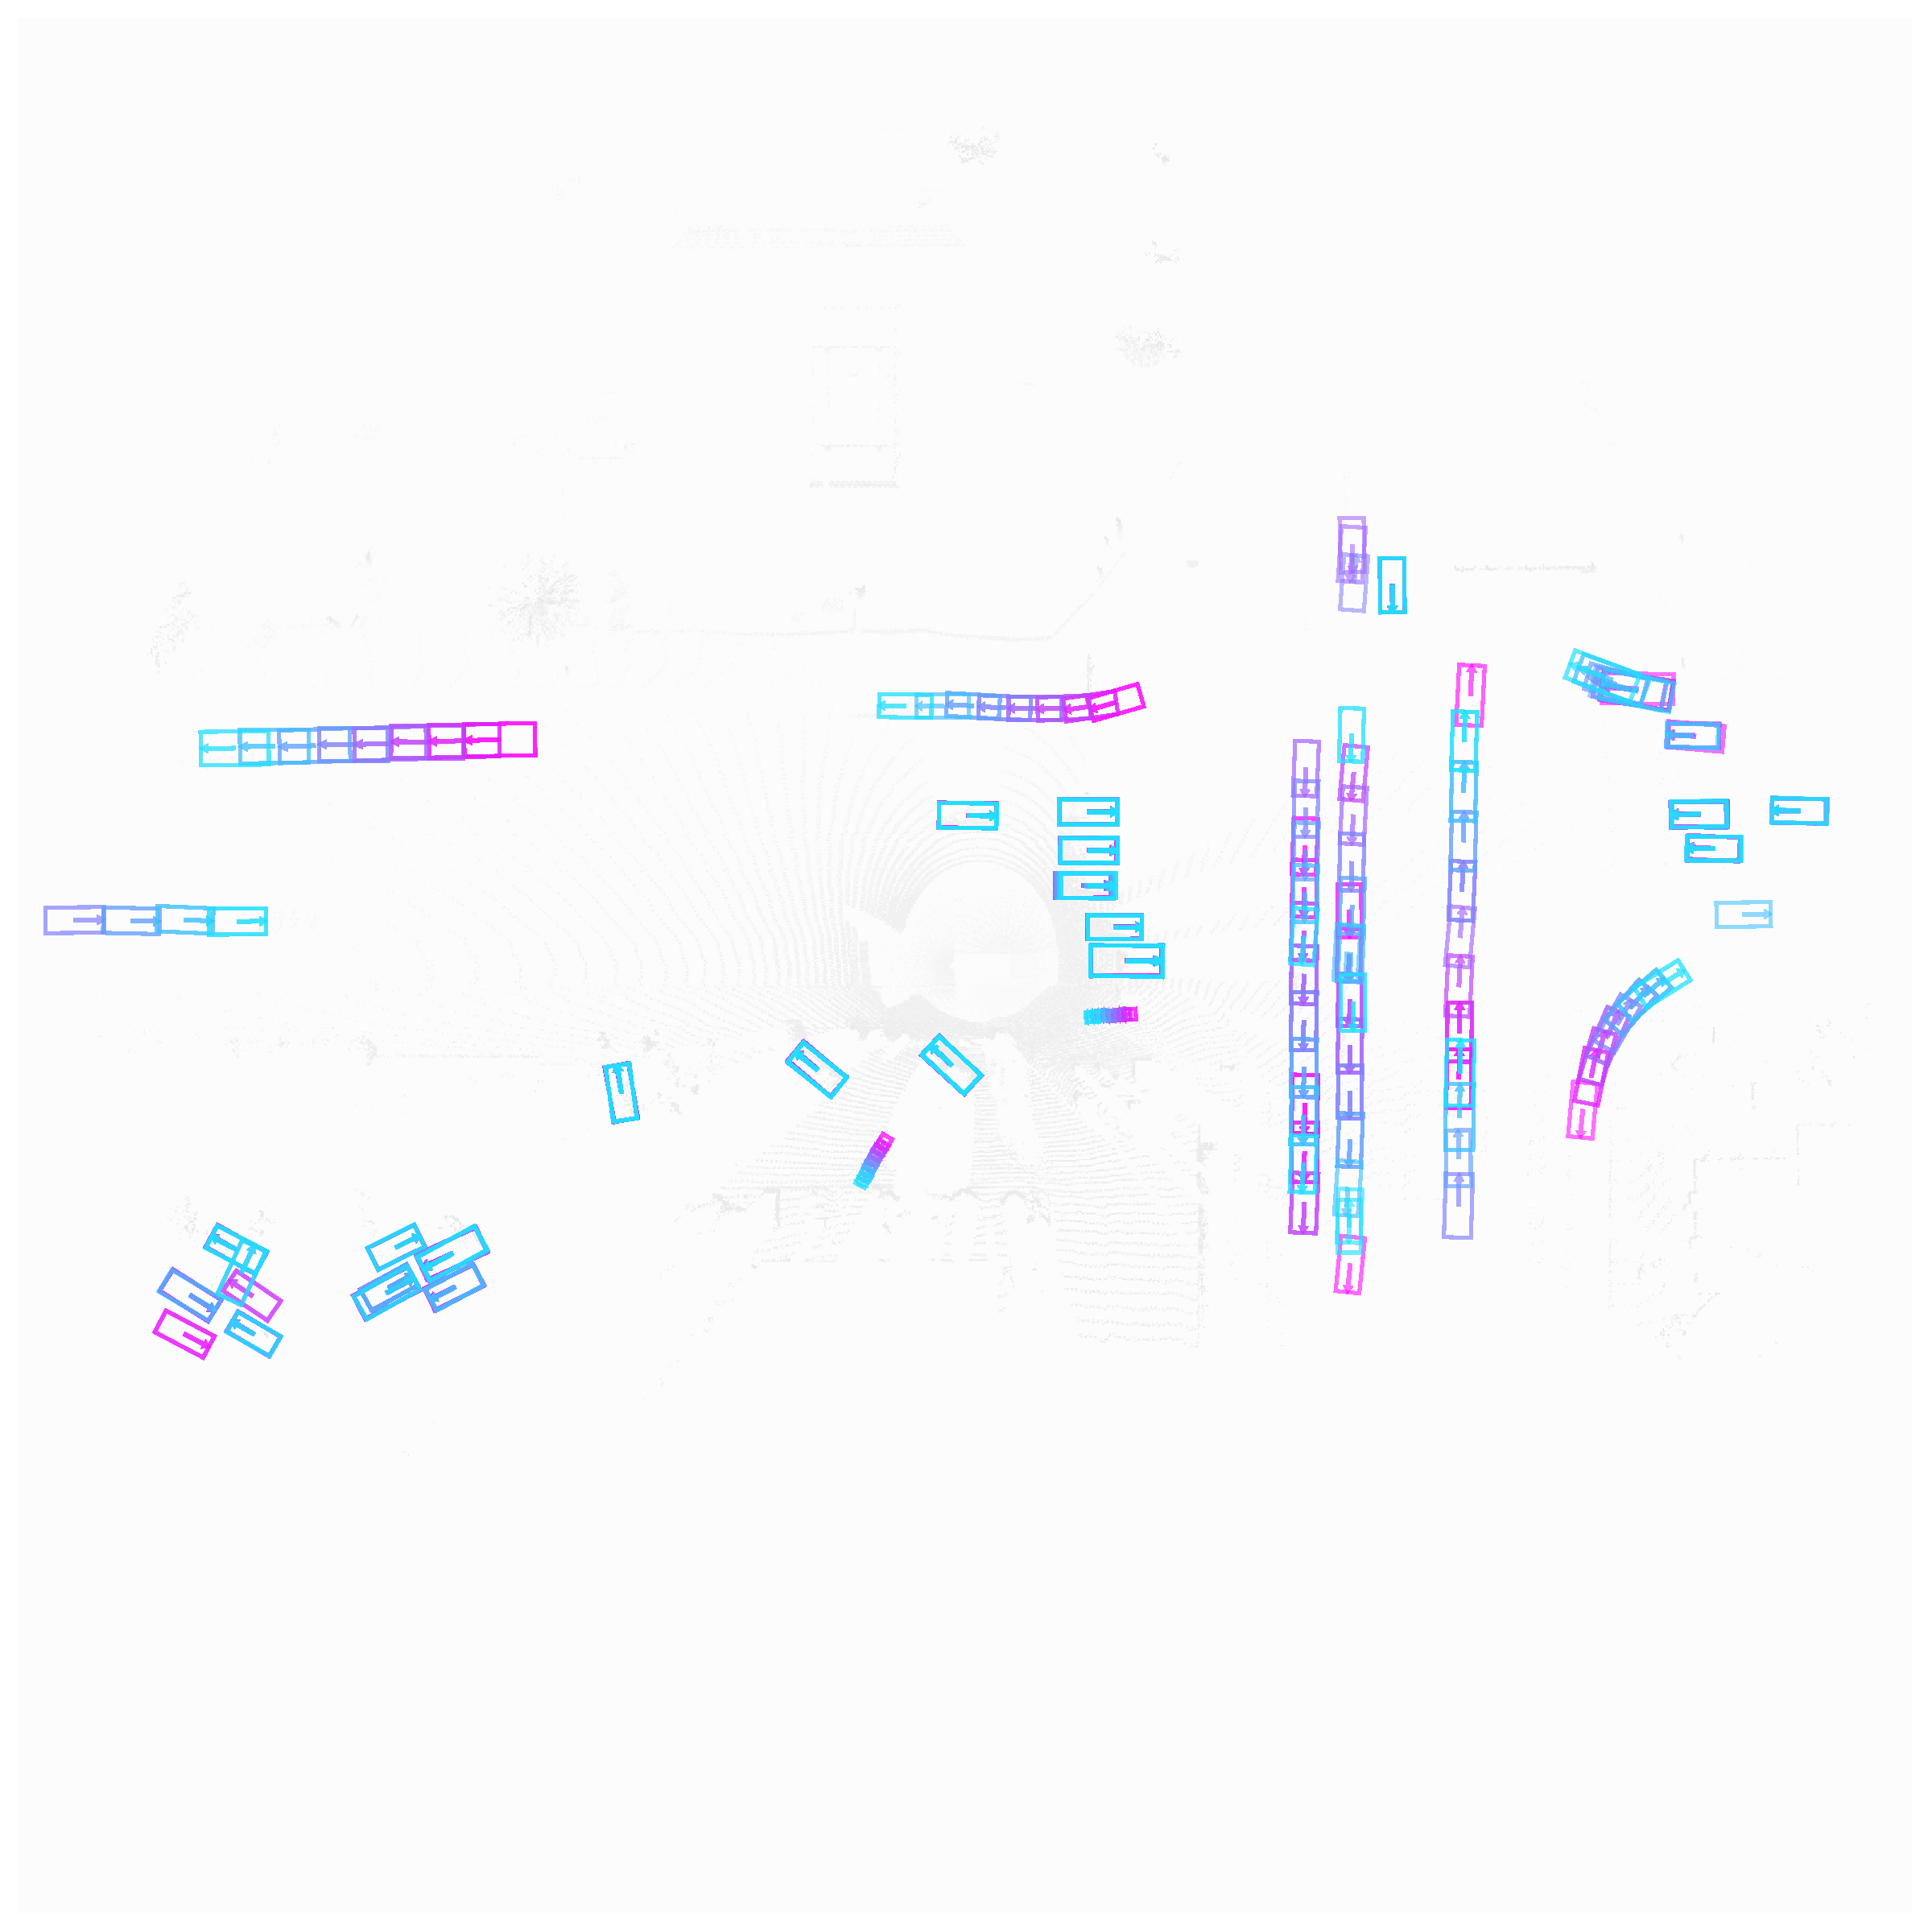
\includegraphics[width=\imw, viewport=72 288 936 1152, clip]{images_for_supp/64/original_det_anchors_wod_viz_64_90.pdf}};
    \node[draw=black,very thick,anchor=west ,inner sep=0pt]  (S3C) at (S3B.east)                   {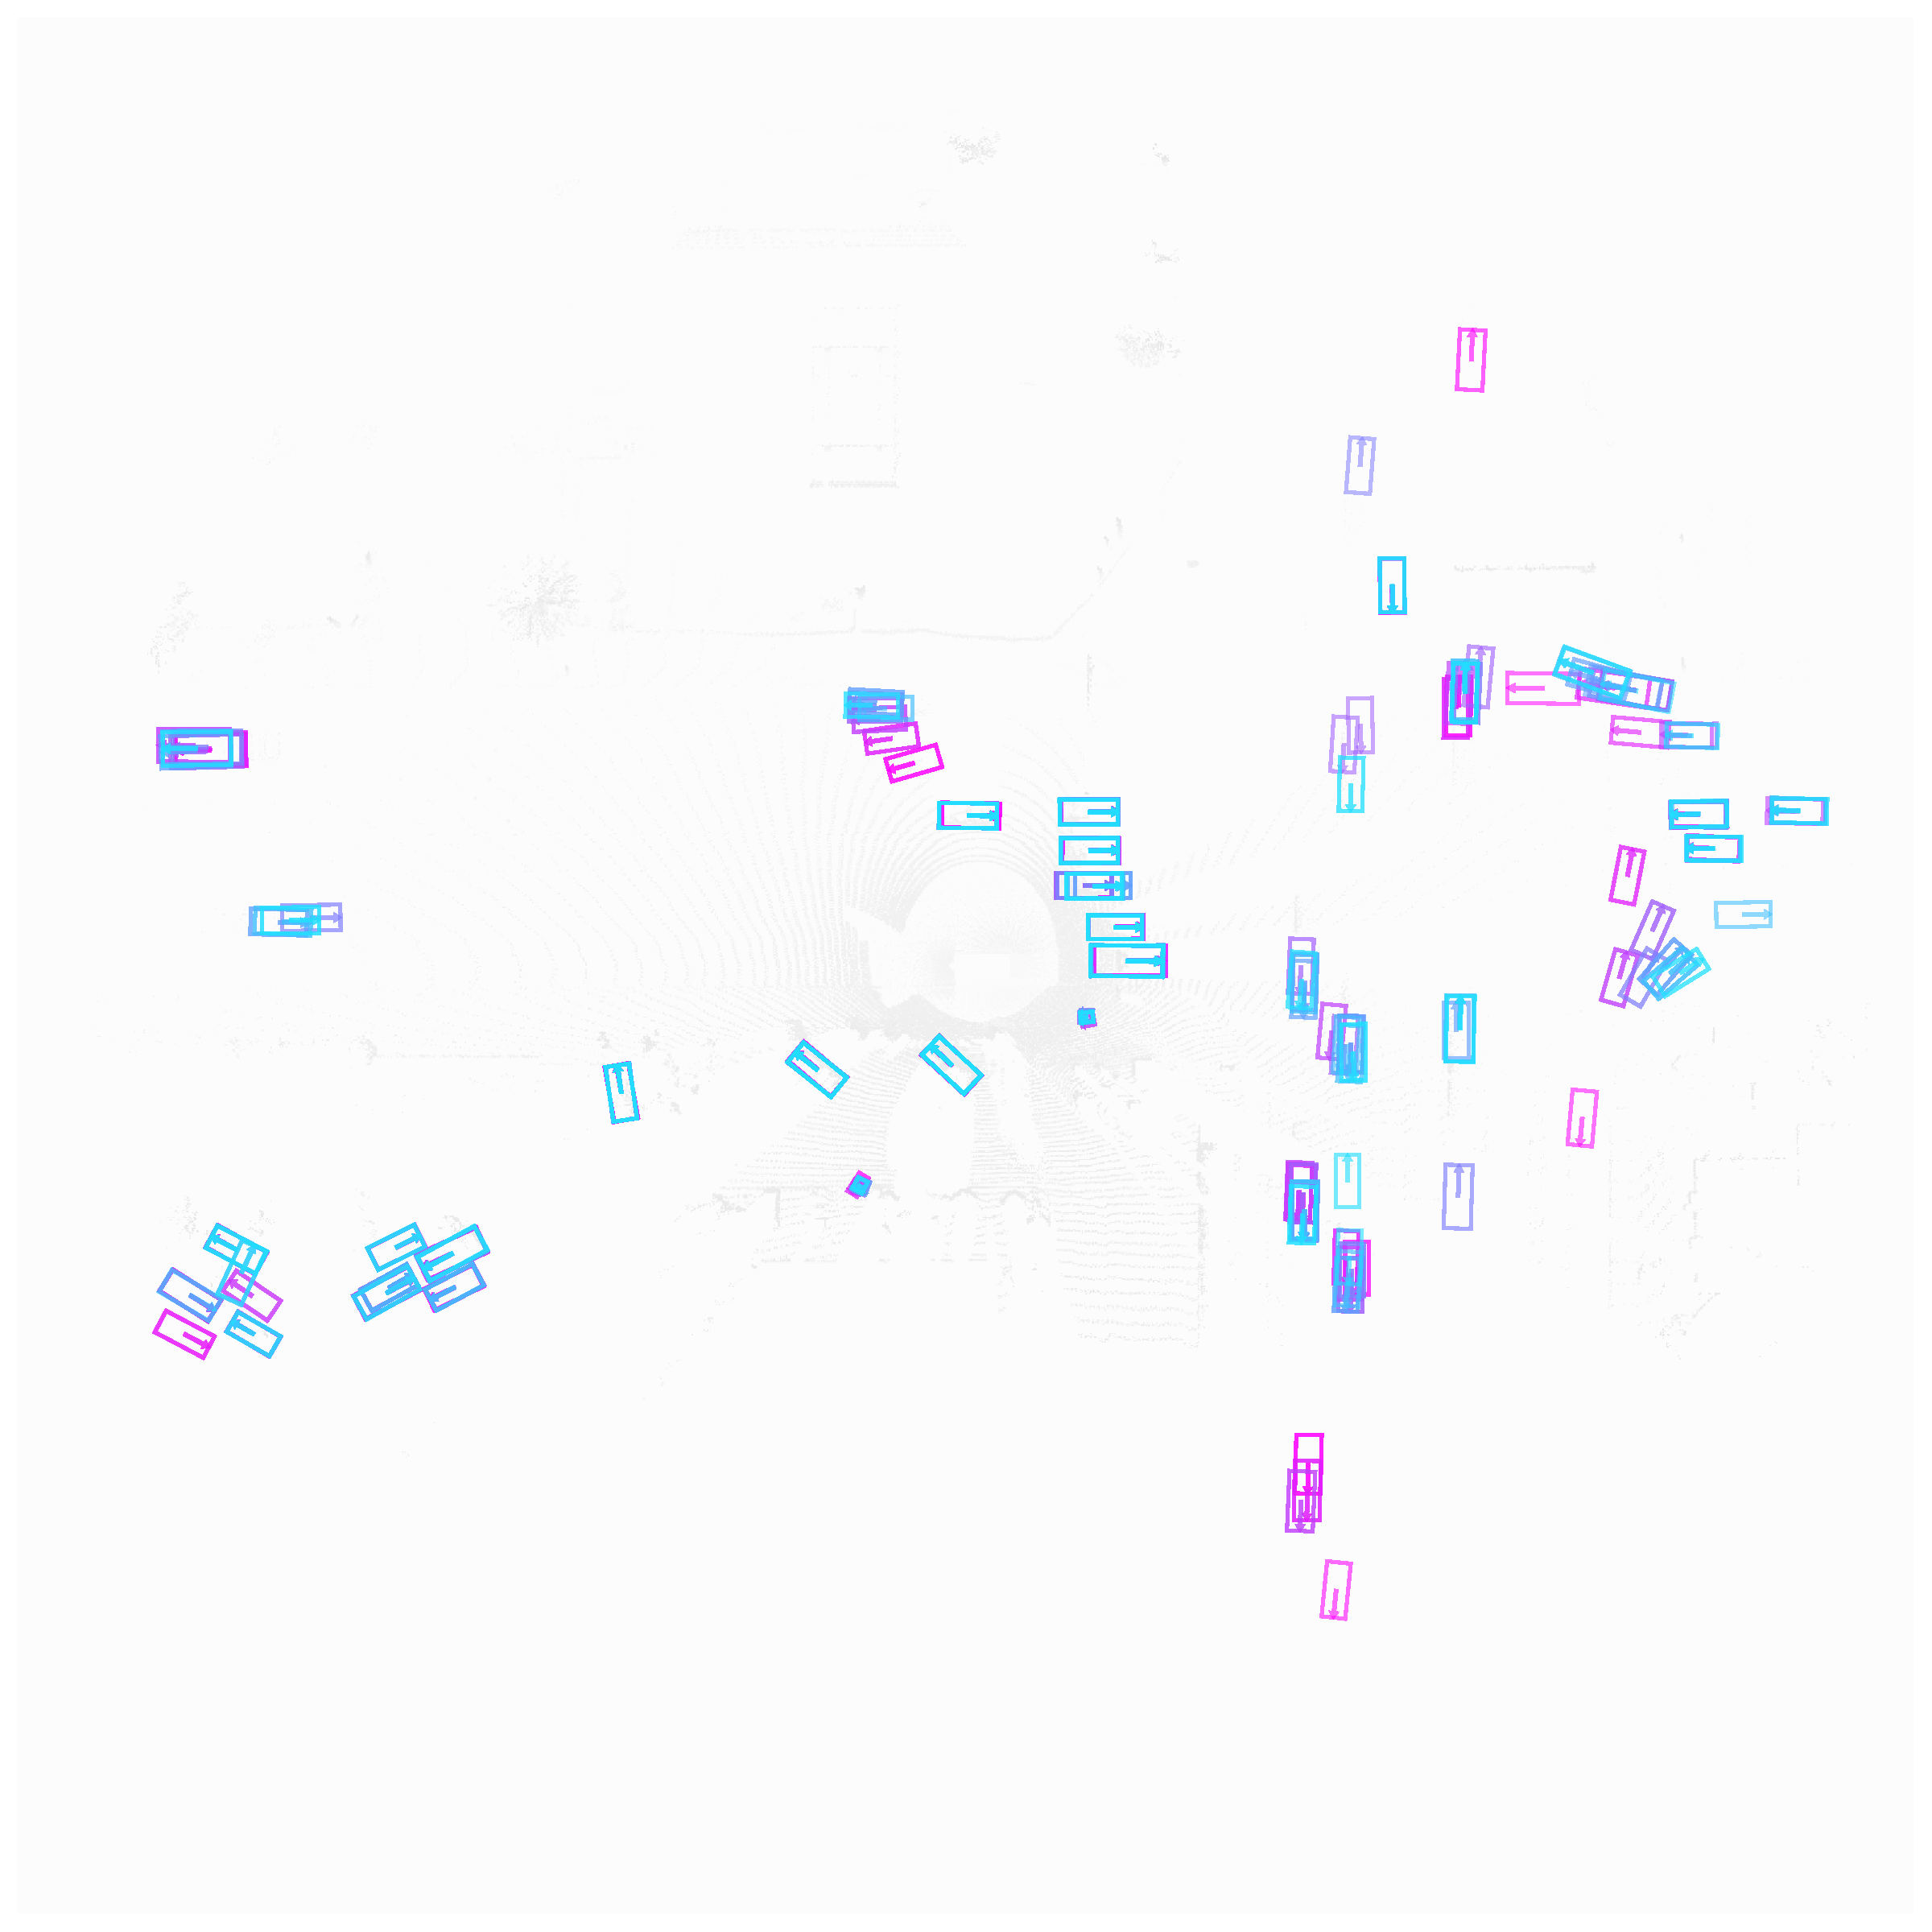
\includegraphics[width=\imw, viewport=72 288 936 1152, clip]{images_for_supp/64/interpolated_det_anchors_wod_viz_64_90.pdf}};
    \node[draw=black,very thick,anchor=west ,inner sep=0pt]  (S3D) at (S3C.east)                   {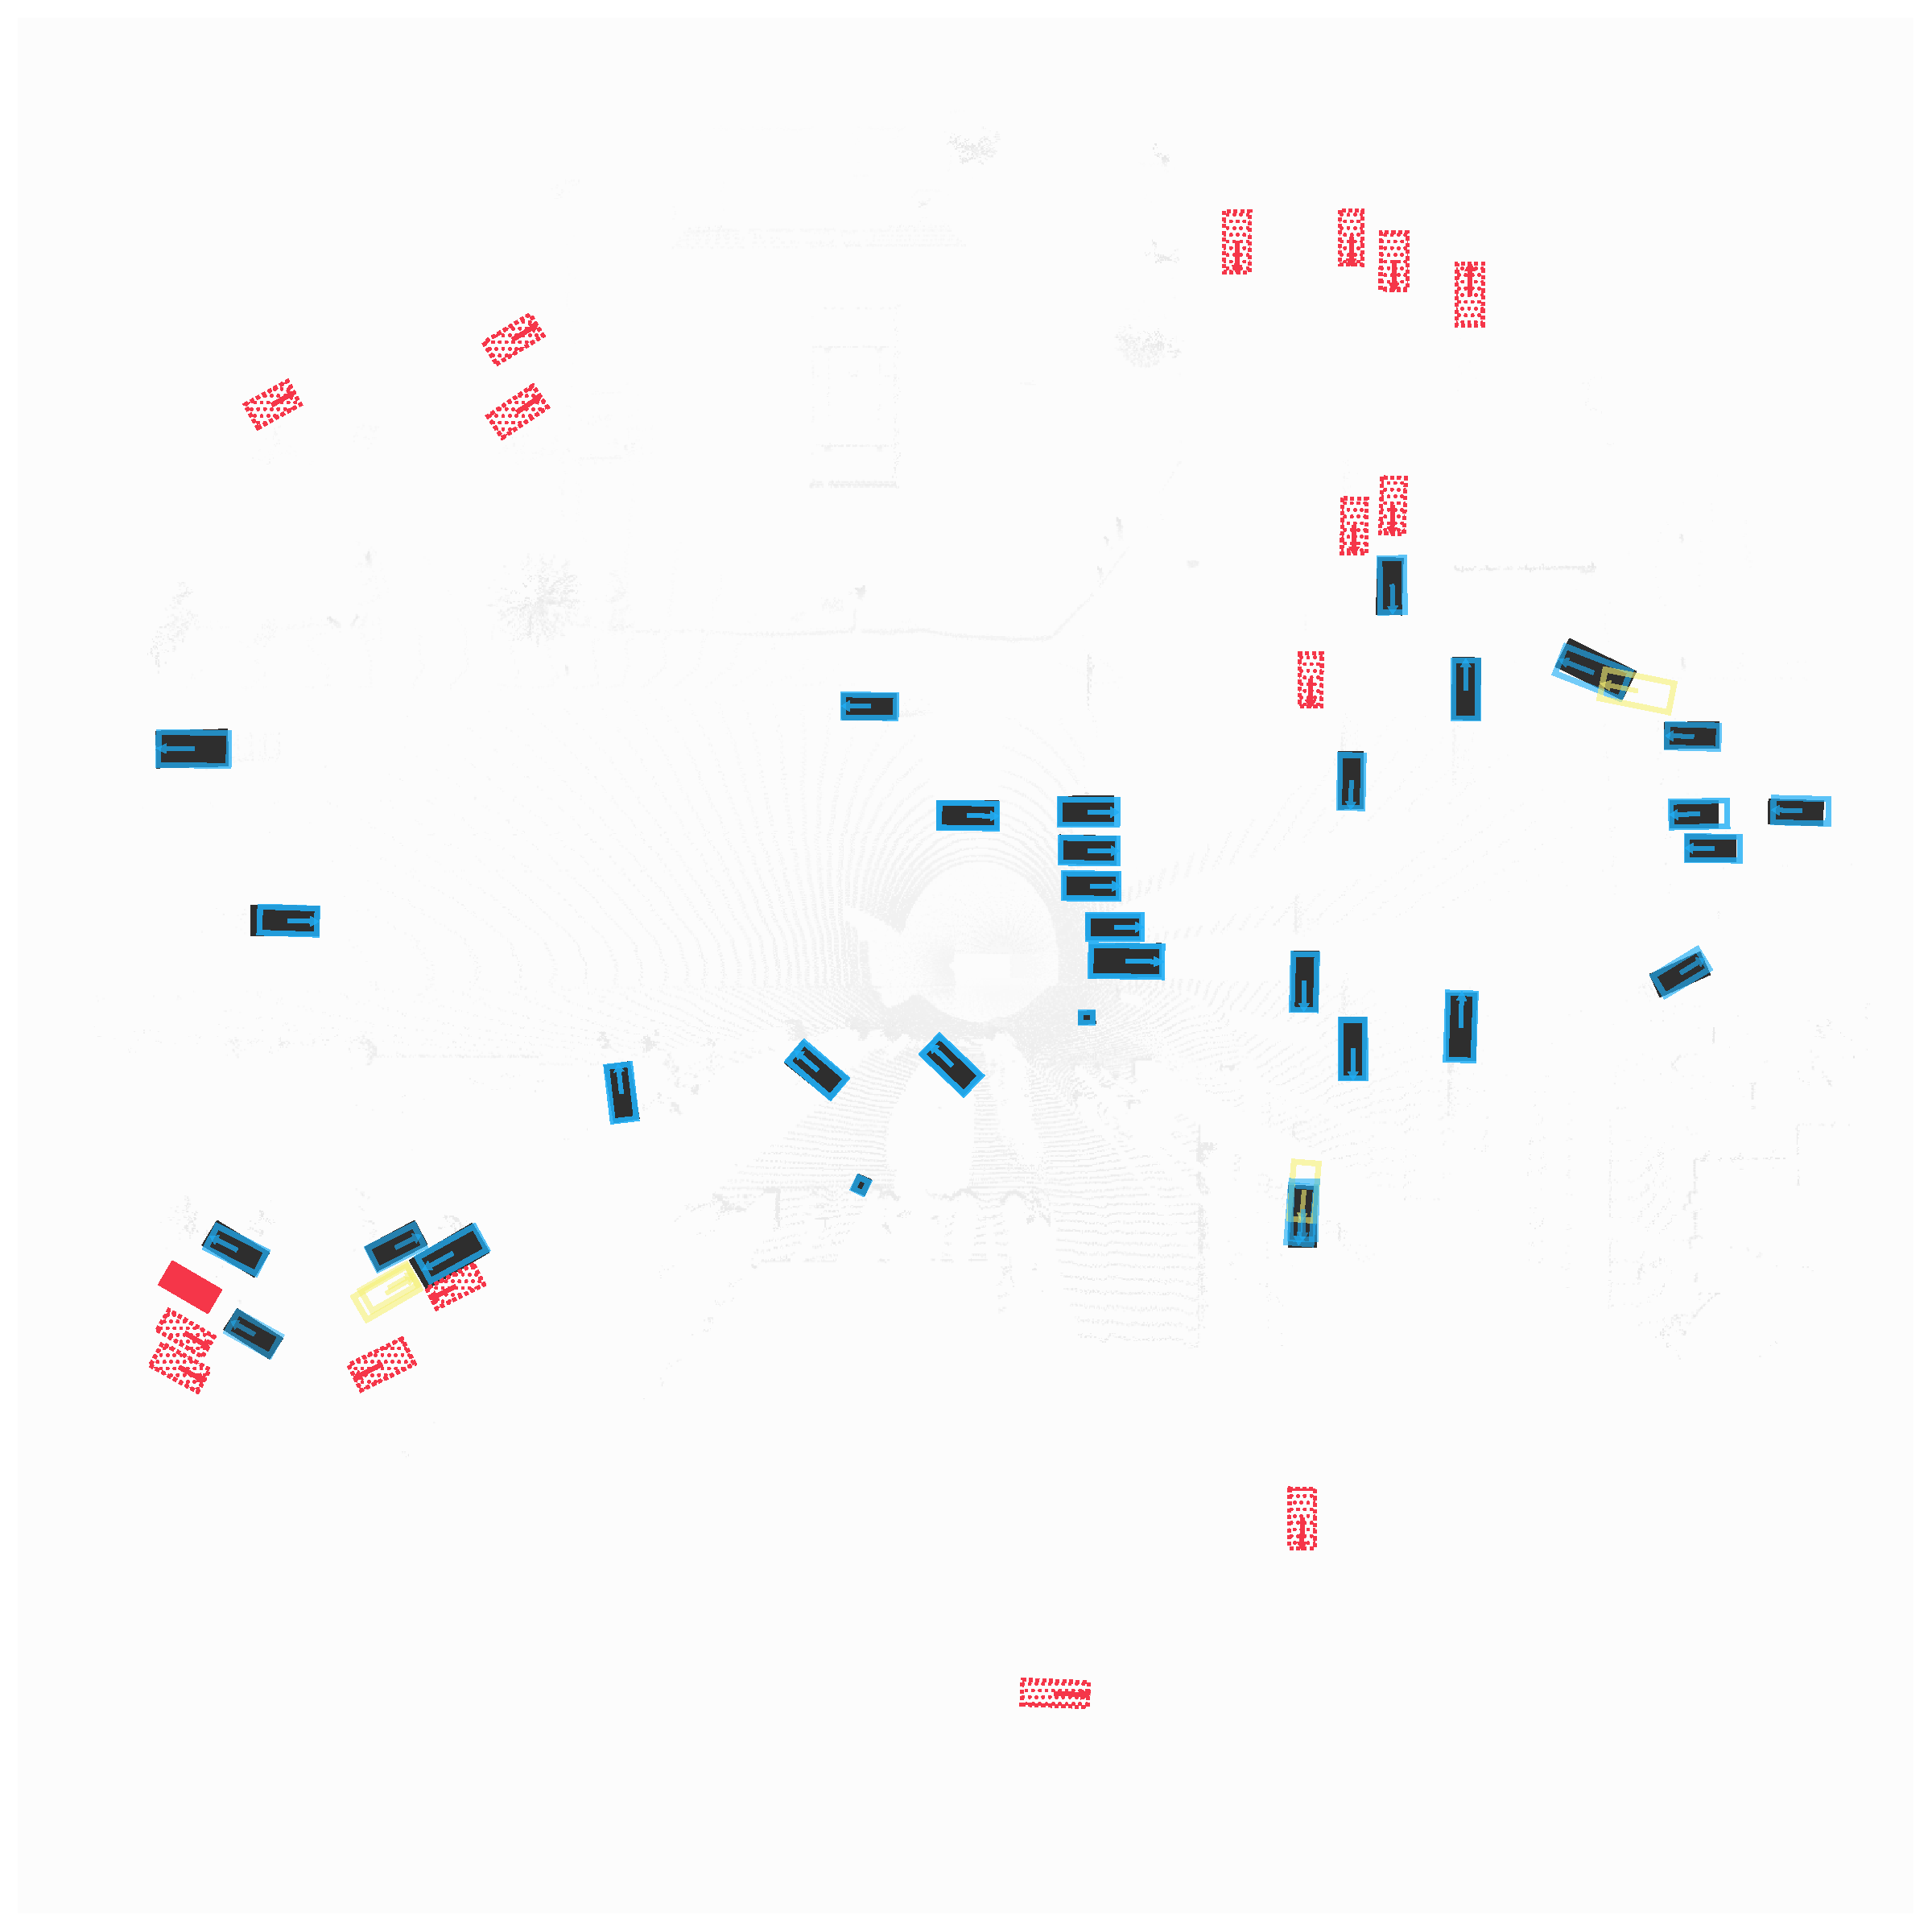
\includegraphics[width=\imw, viewport=72 288 936 1152, clip]{images_for_supp/64/detections_wod_viz_64_90.pdf}};

    \node[draw=black,very thick,anchor=north, inner sep=0pt] (S4A) at ([yshift=-\rowsep]S3A.south) {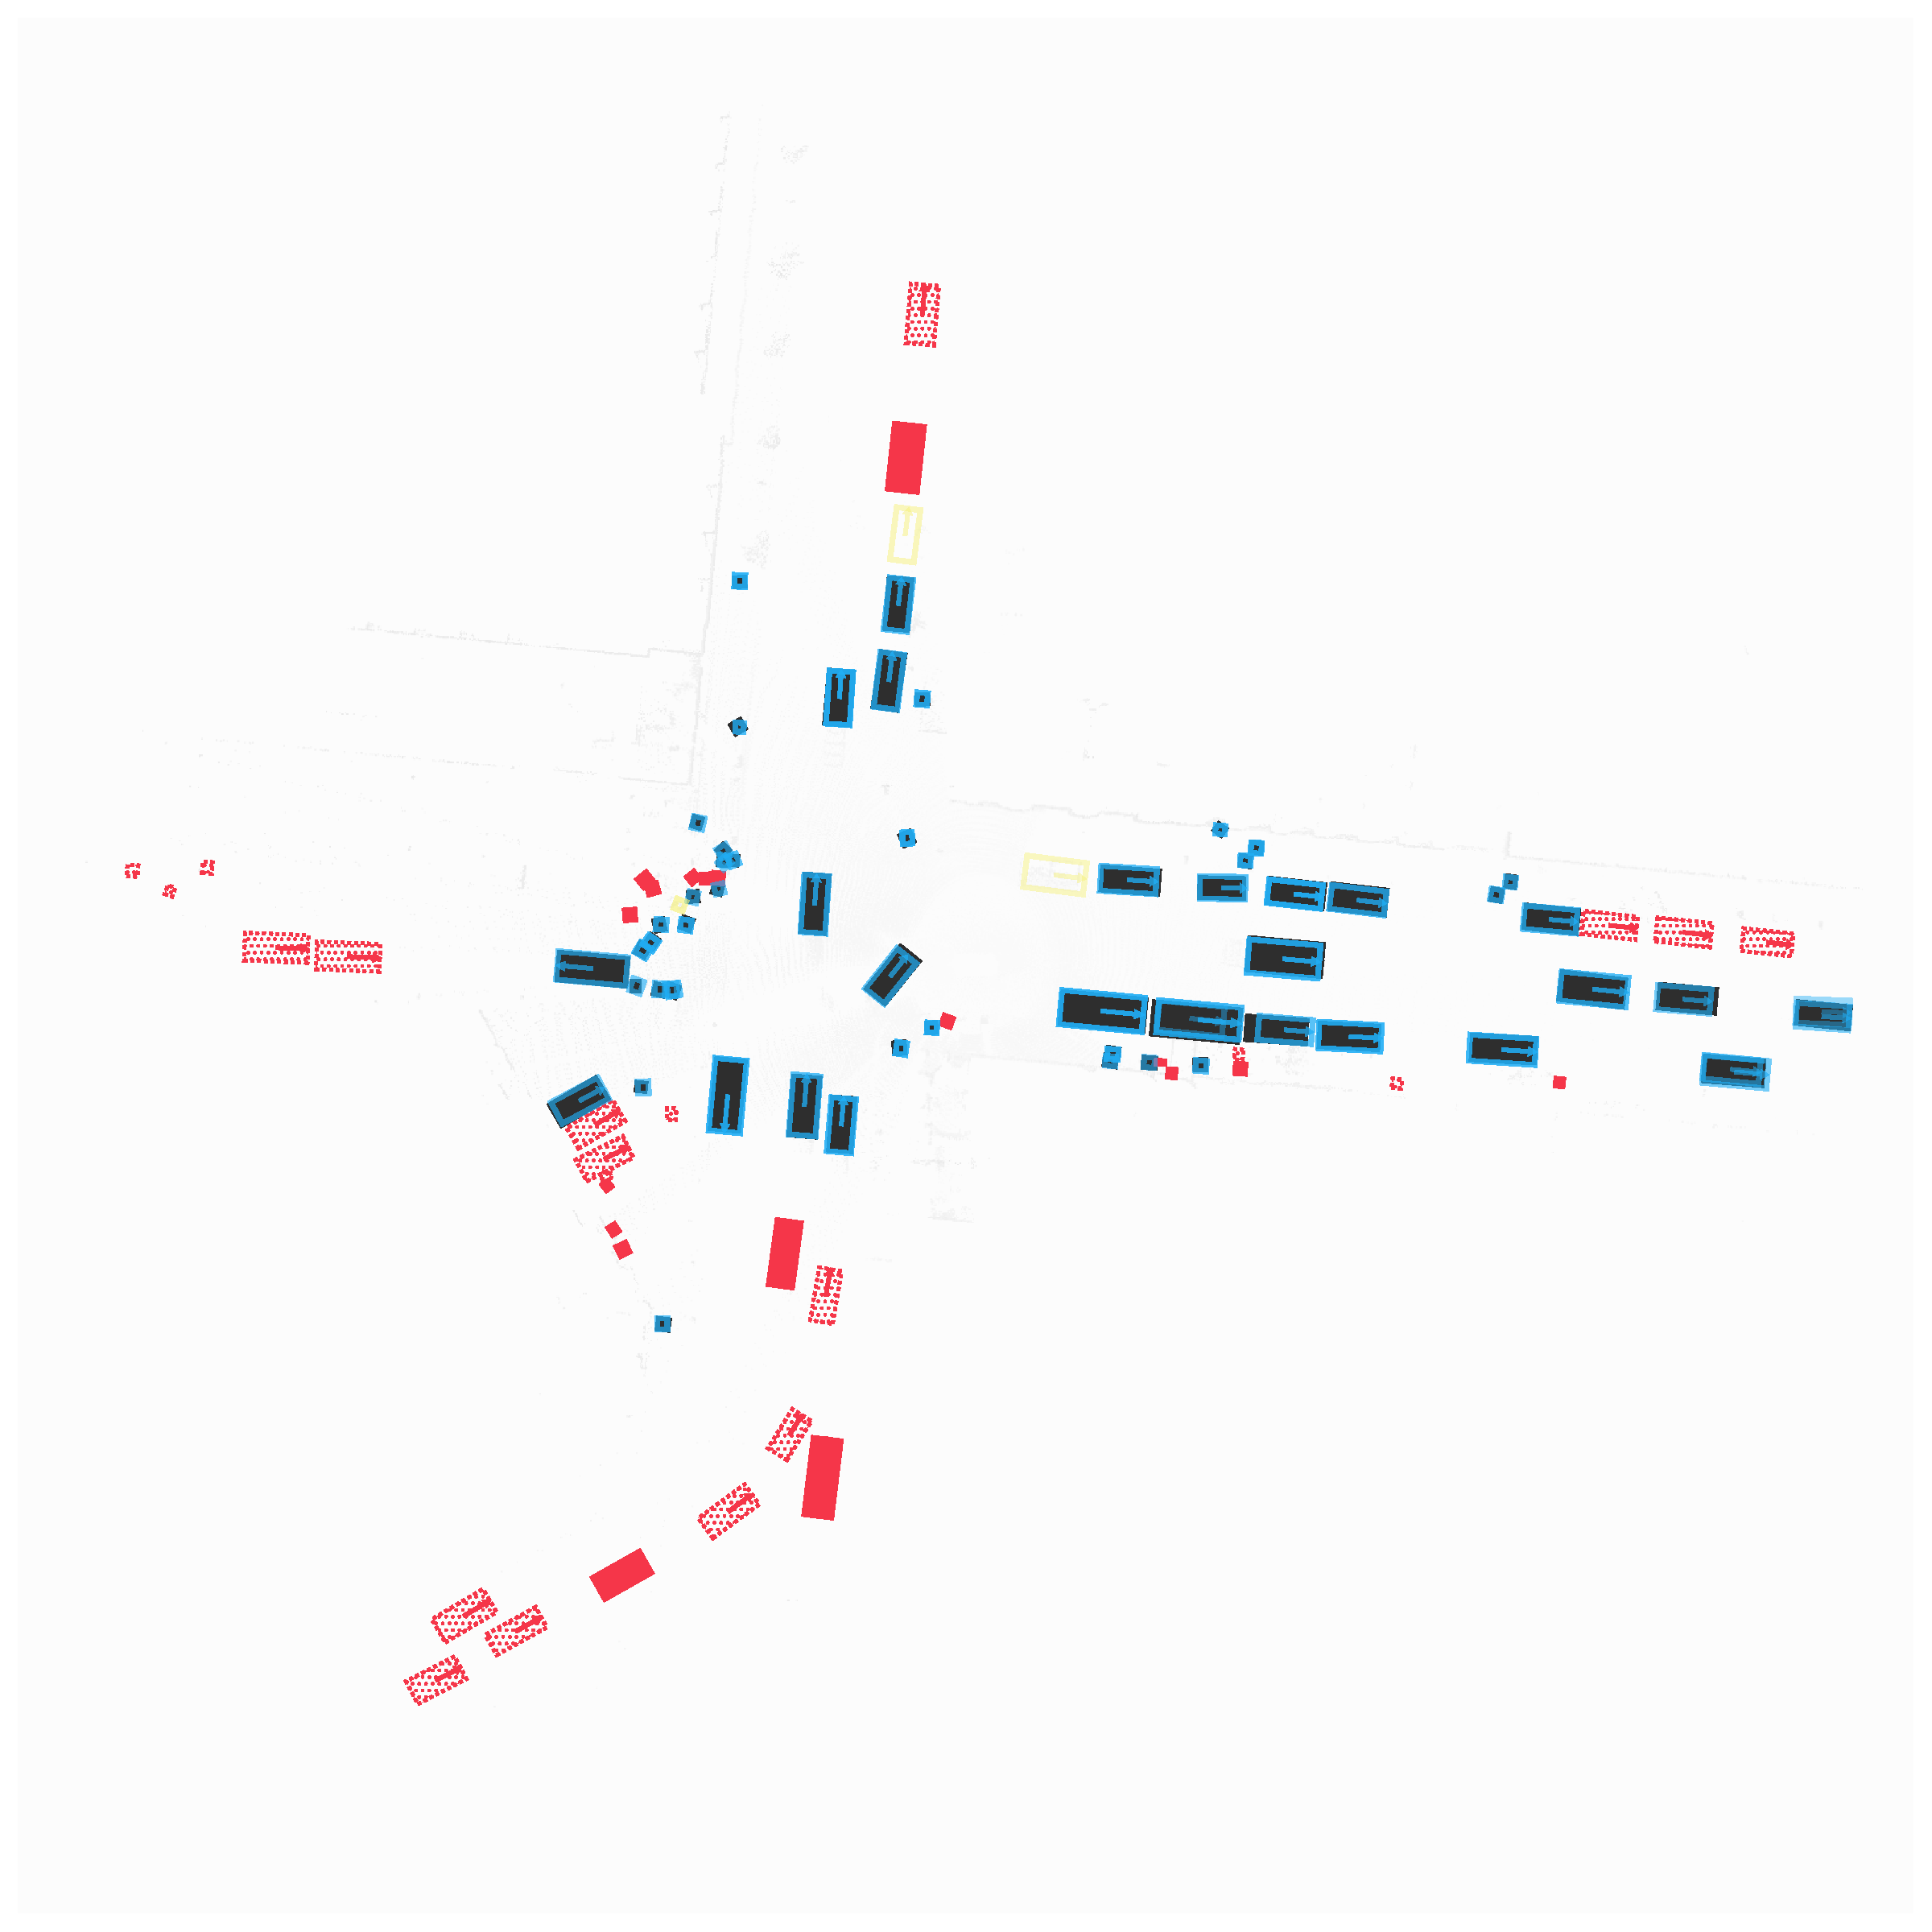
\includegraphics[width=\imw, viewport=144 144 936 936, clip]{images_for_supp/73/lidar_proposals_wod_viz_73_126.pdf}};
    \node[draw=black,very thick,anchor=west , inner sep=0pt]  (S4B) at (S4A.east)                   {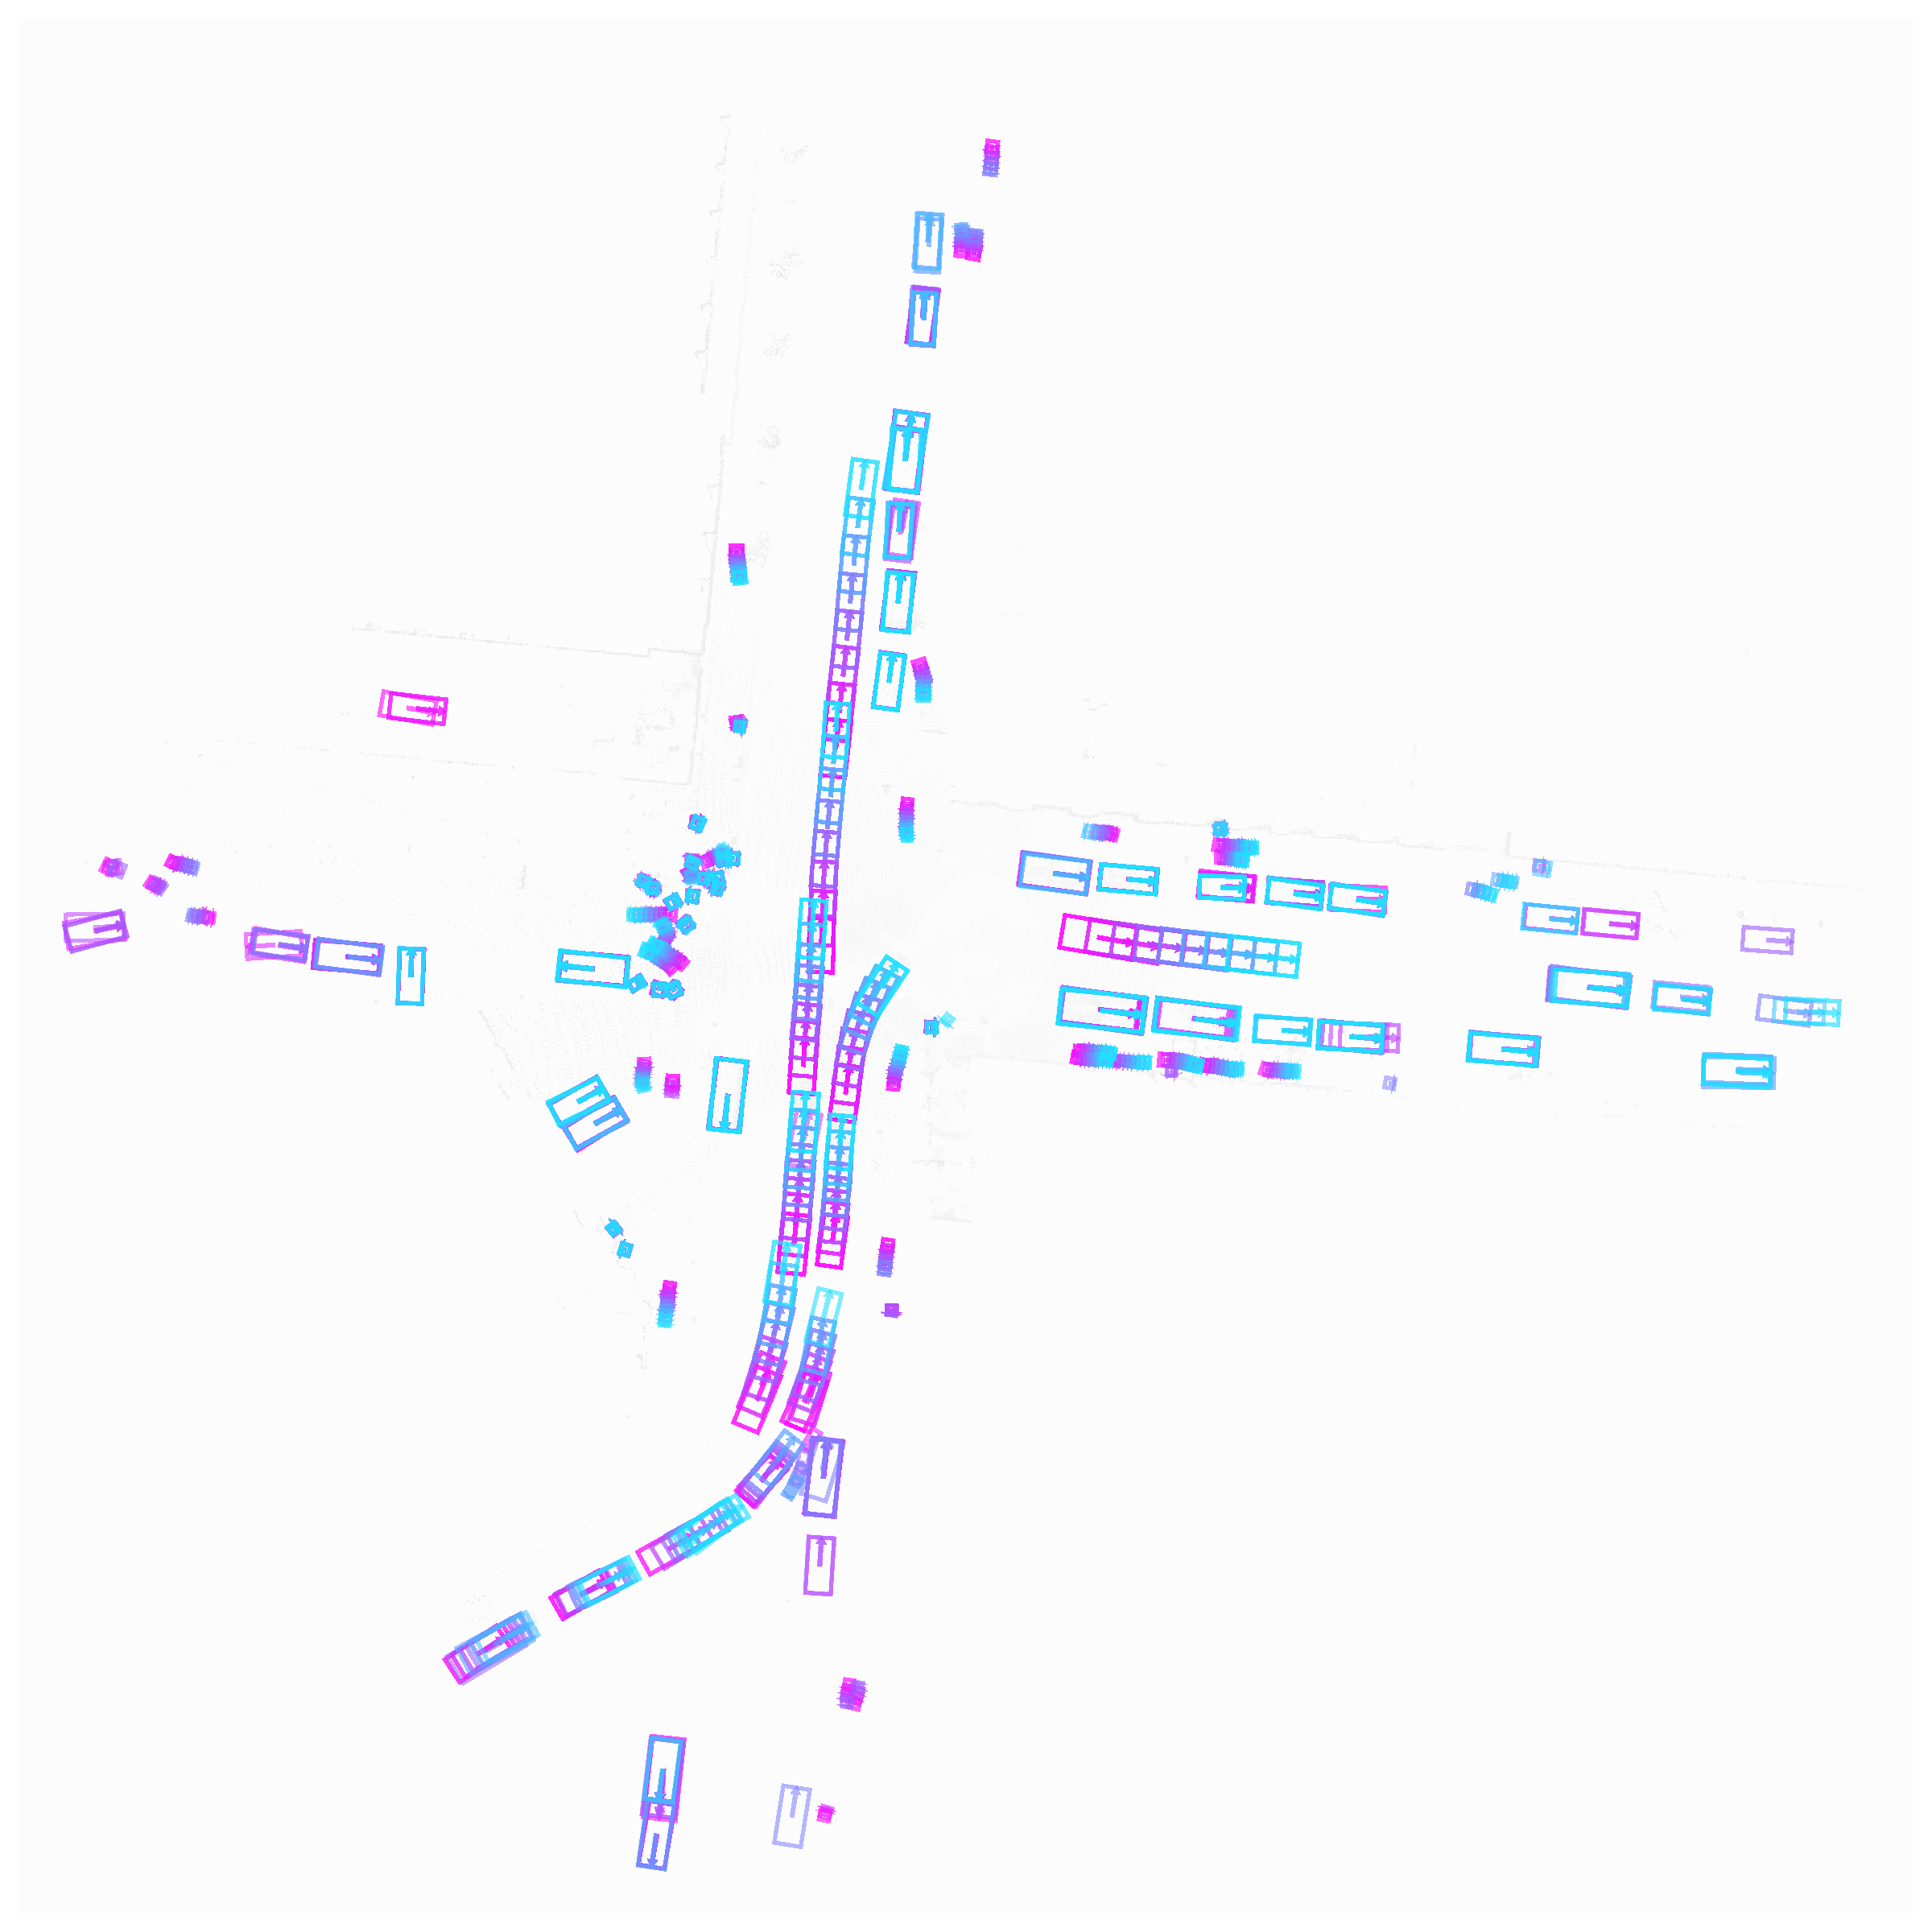
\includegraphics[width=\imw, viewport=144 144 936 936, clip]{images_for_supp/73/original_det_anchors_wod_viz_73_126.pdf}};
    \node[draw=black,very thick,anchor=west , inner sep=0pt]  (S4C) at (S4B.east)                   {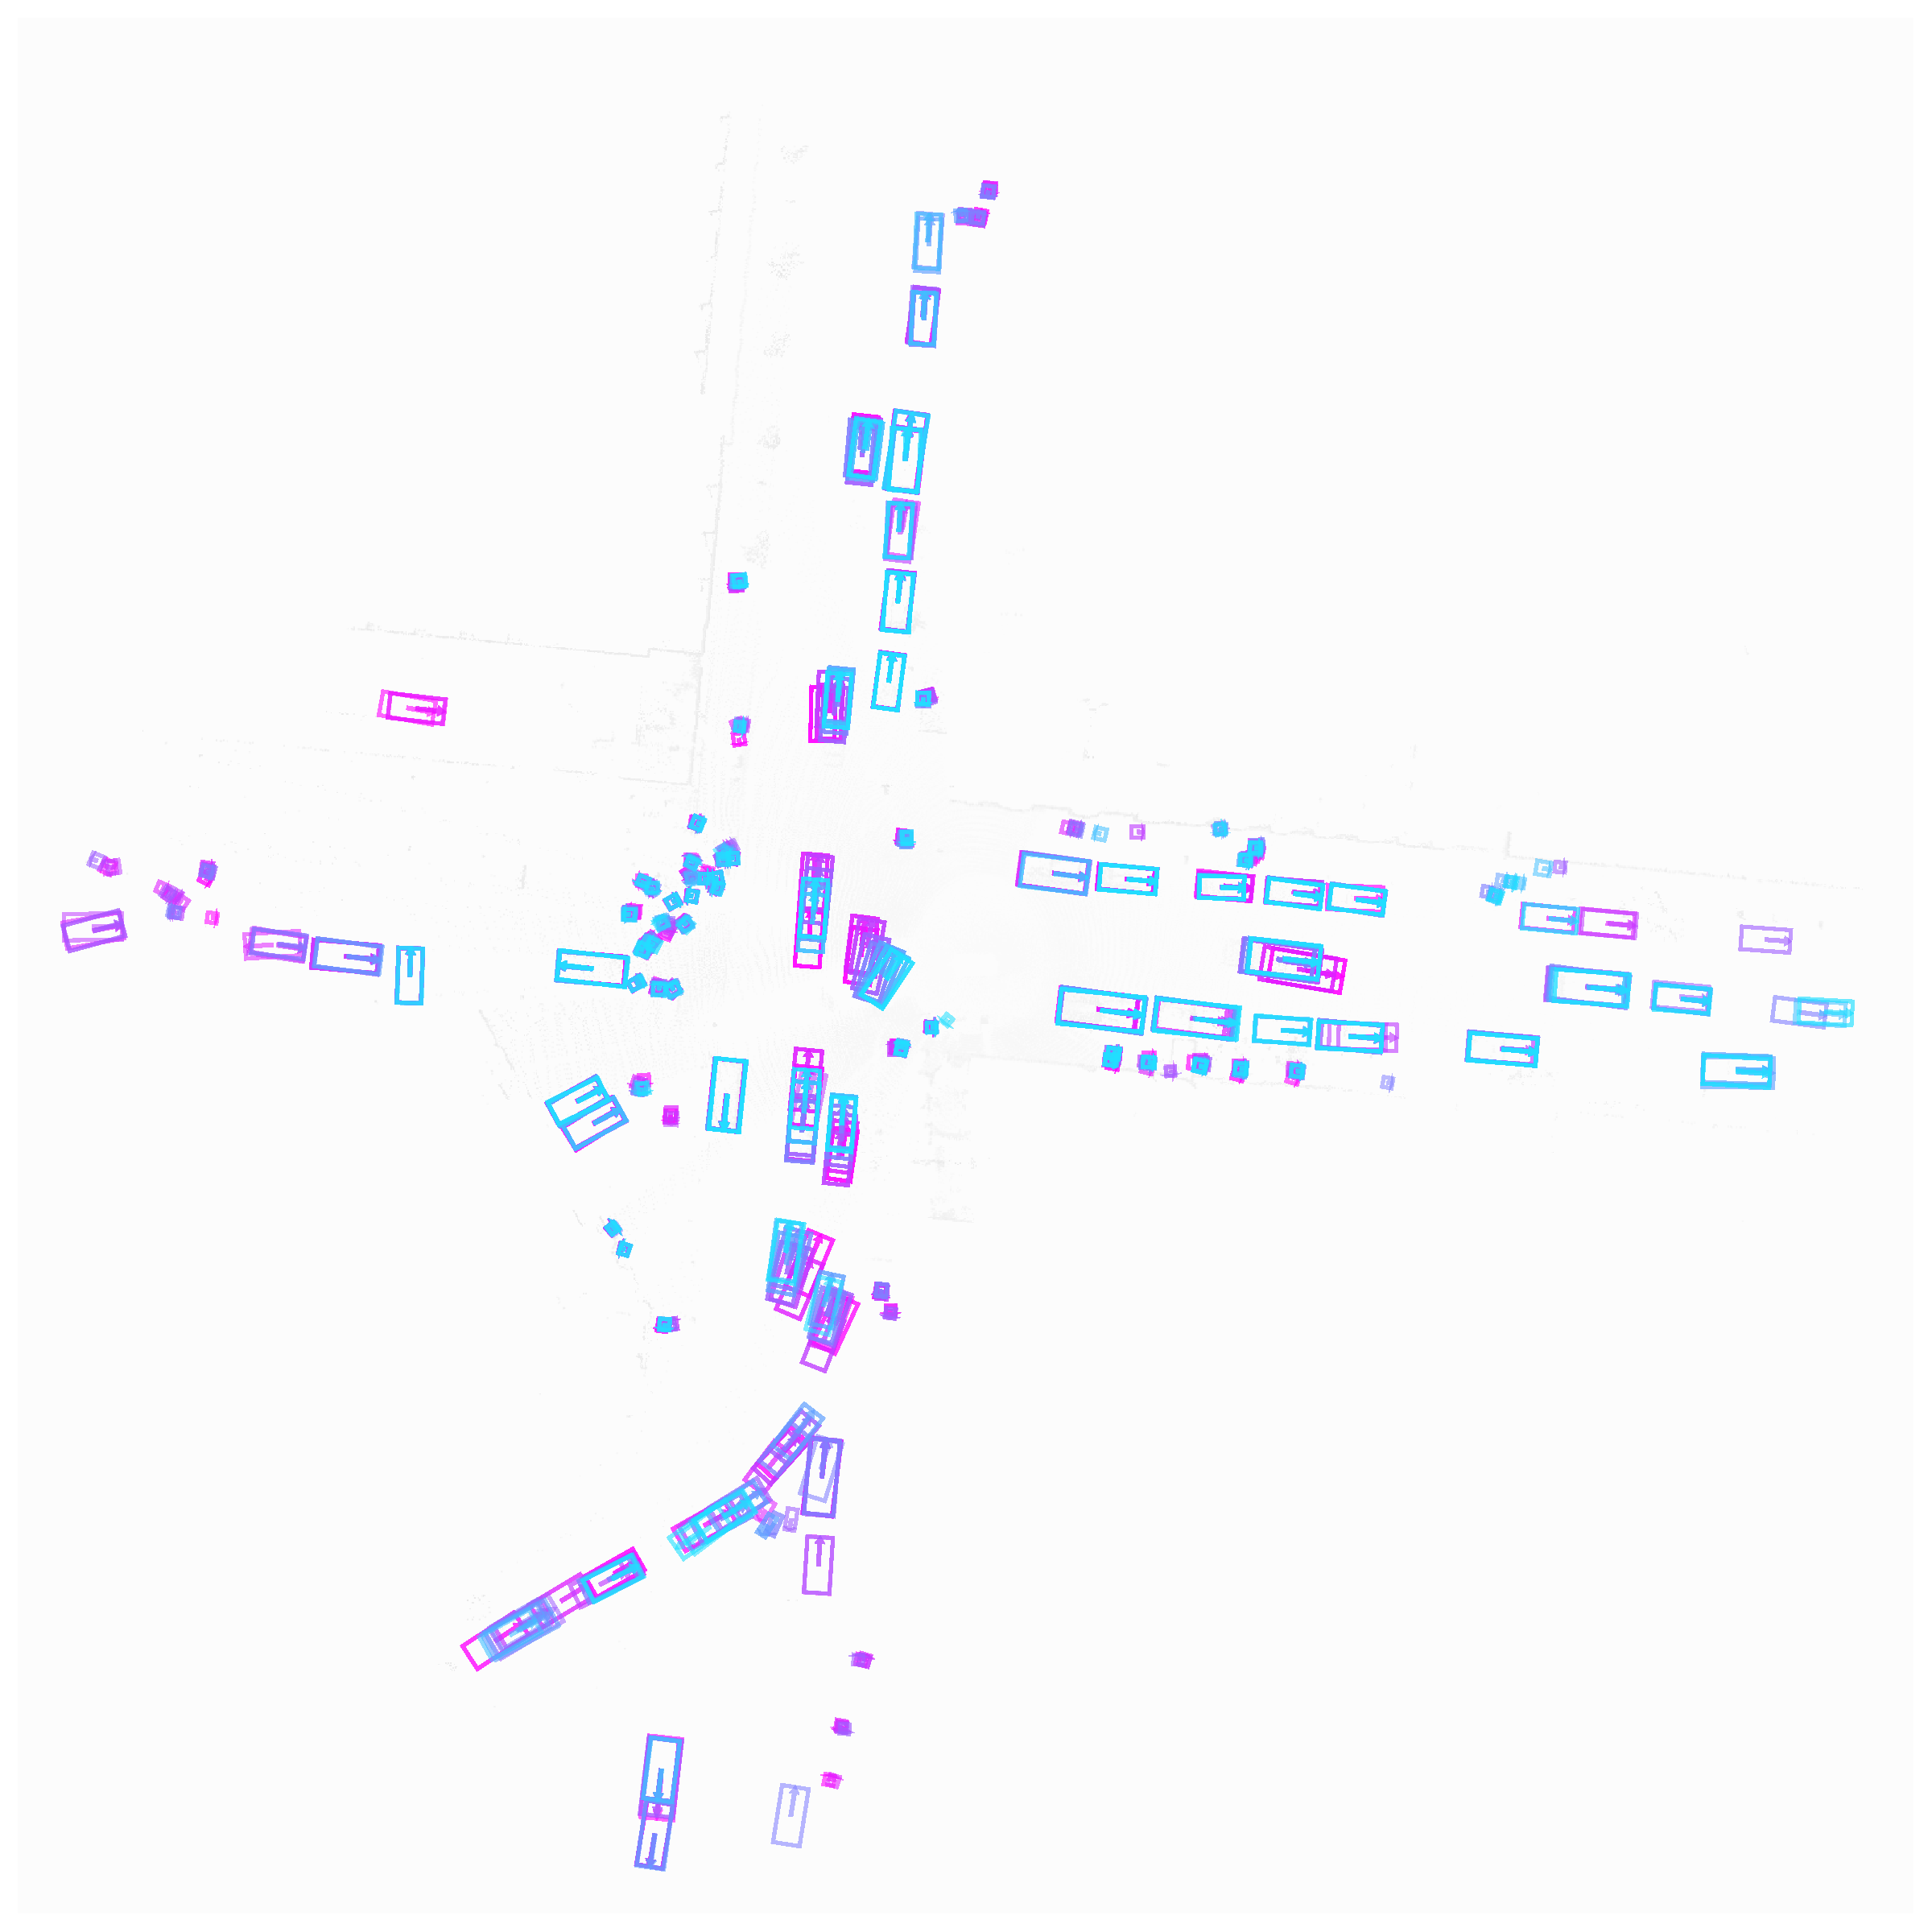
\includegraphics[width=\imw, viewport=144 144 936 936, clip]{images_for_supp/73/interpolated_det_anchors_wod_viz_73_126.pdf}};
    \node[draw=black,very thick,anchor=west , inner sep=0pt]  (S4D) at (S4C.east)                   {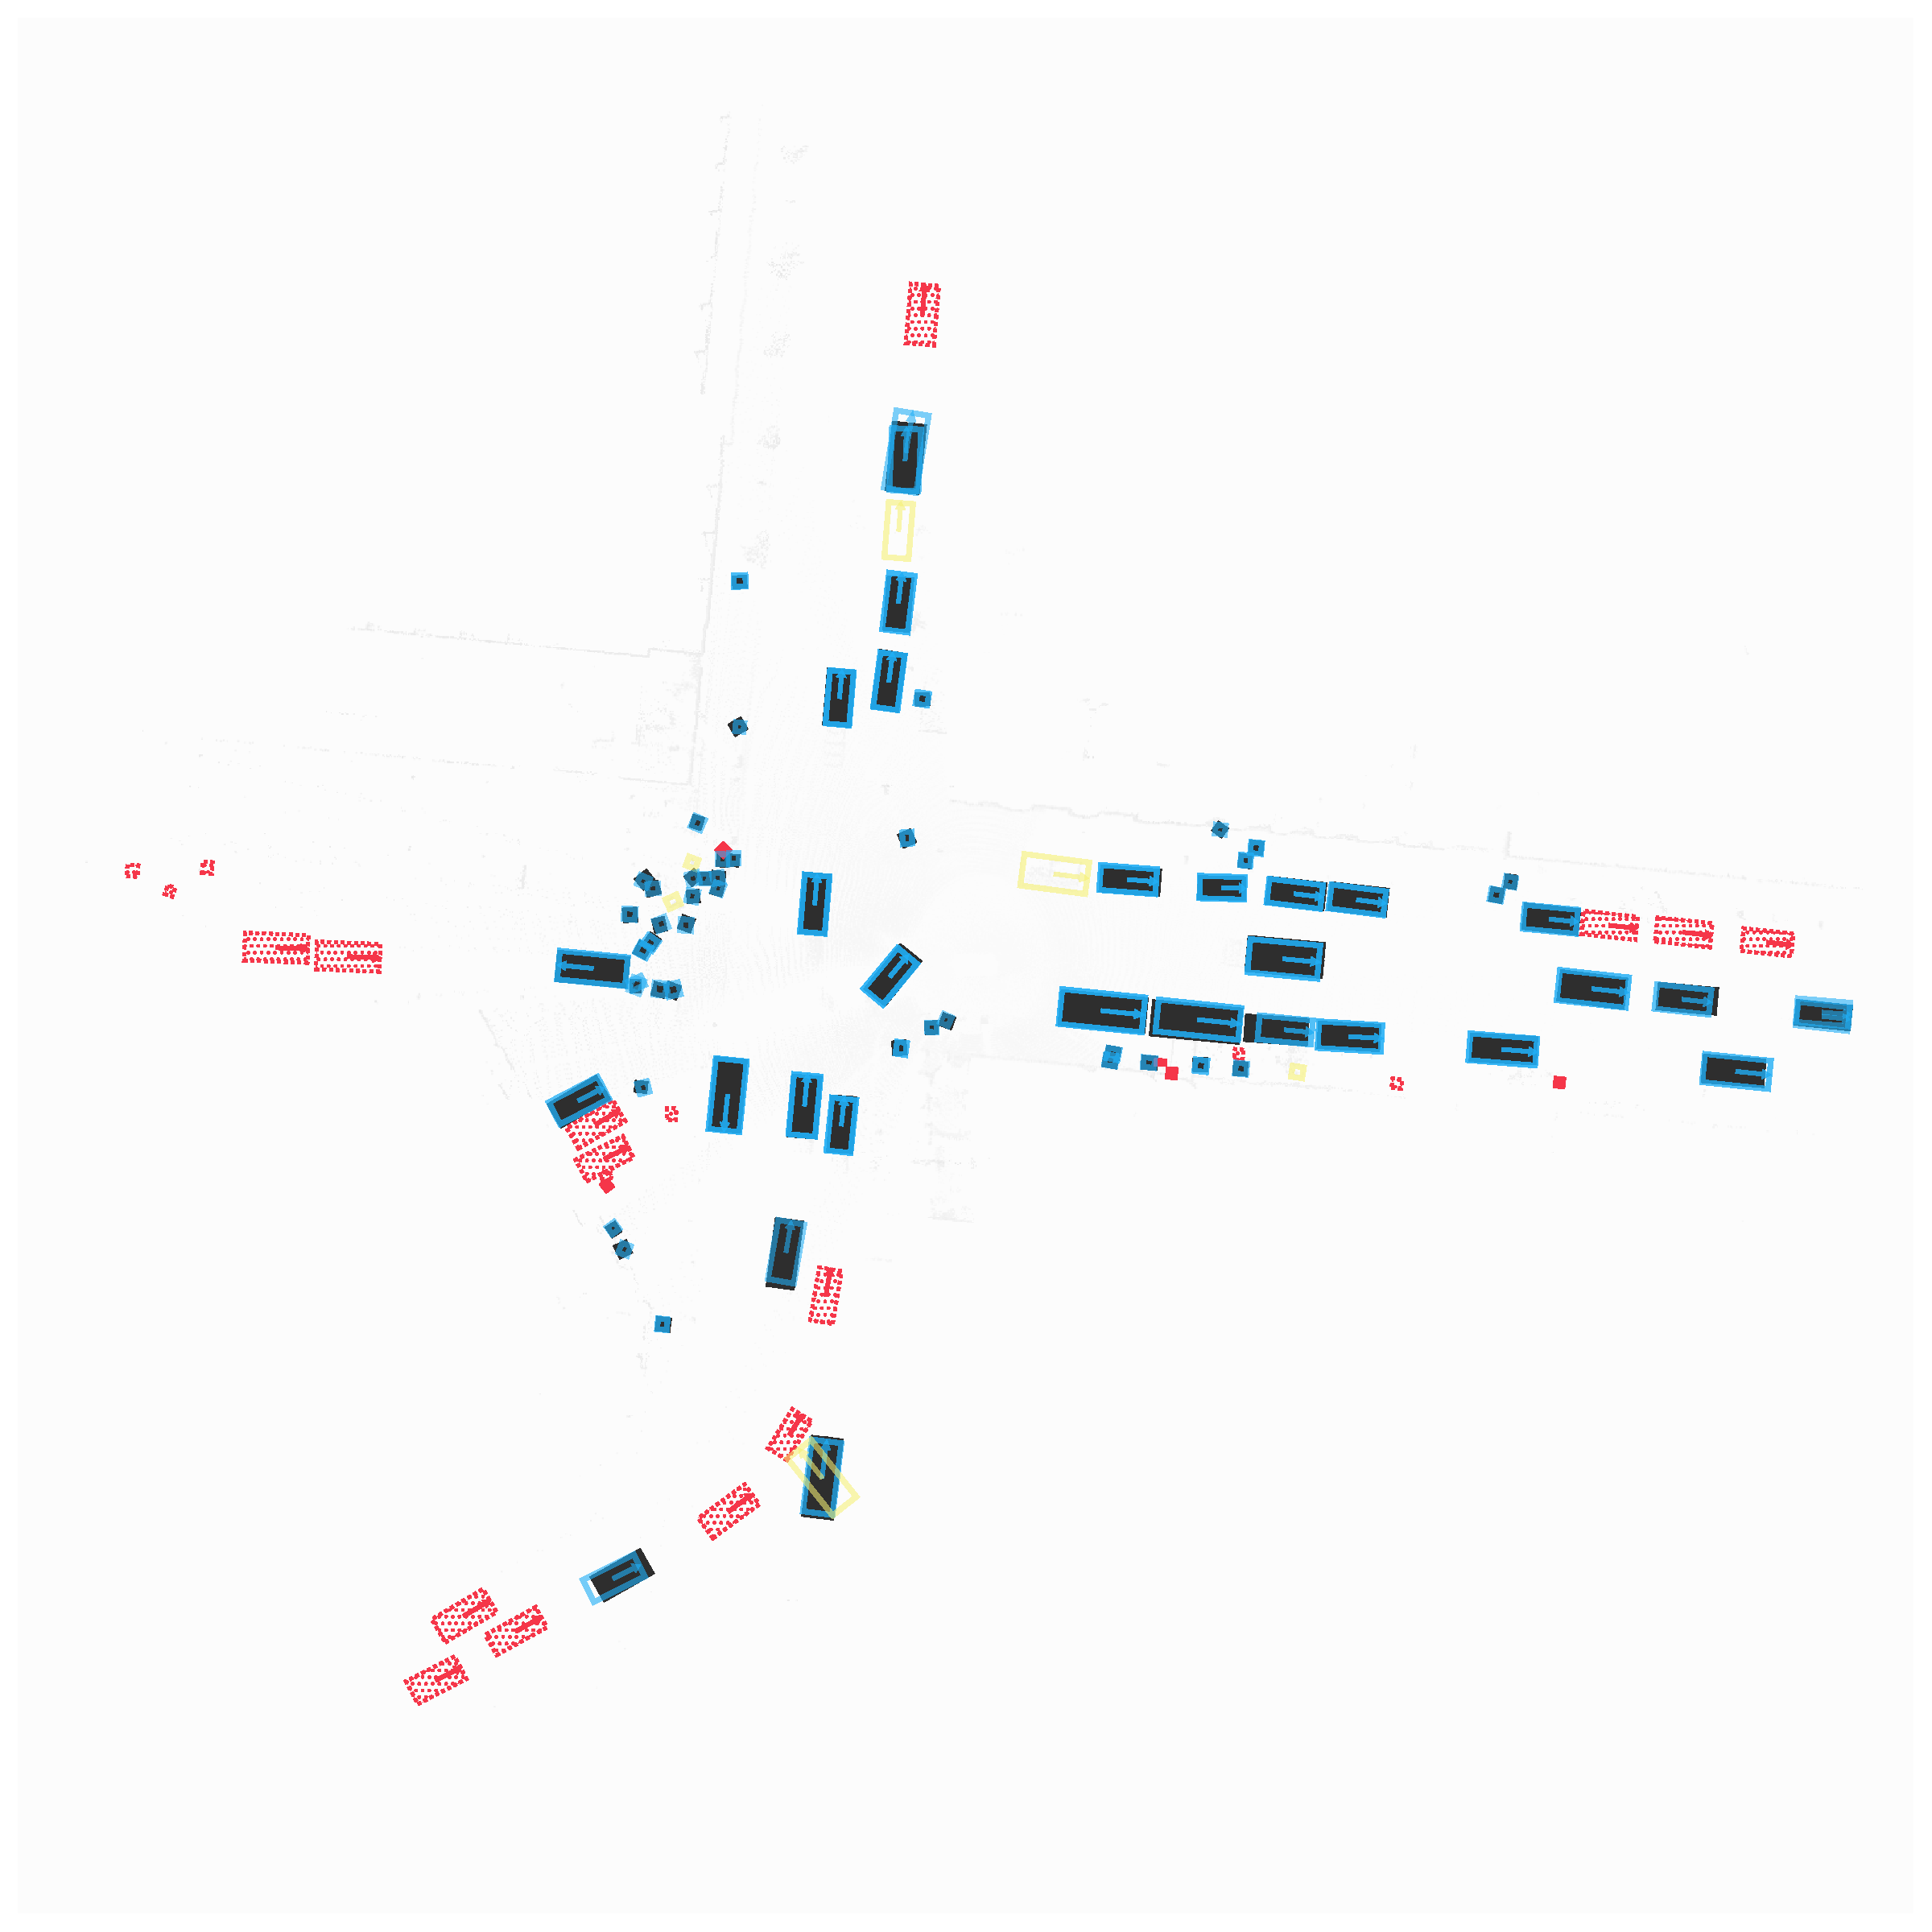
\includegraphics[width=\imw, viewport=144 144 936 936, clip]{images_for_supp/73/detections_wod_viz_73_126.pdf}};

    % Labels for rows (Scenes)
    % \node[anchor=south,rotate=90] at (S1A.west) {Scene \#1};
    % \node[anchor=south,rotate=90] at (S2A.west) {Scene \#2};
    % \node[anchor=south,rotate=90] at (S3A.west) {Scene \#3};
    % \node[anchor=south,rotate=90] at (S4A.west) {Scene \#4};

    % colormap
    % \node[inner sep=0pt,anchor=north] (cmap) at ($(S1B.north)+(0,-0.2em)$)
    %     {
\includegraphics[width=\imw, height=0.8em, trim={2mm, 2mm, 2mm, 2mm}, clip, angle=180]{images_for_hook_light/cool_colormap.png}};
    % \node[inner sep=0pt,anchor=east] (0) at ([xshift=-0.1em]cmap.east) {\footnotesize 0.0s};
    % \node[inner sep=0pt,anchor=west] (1) at ([xshift=0.1em]cmap.west) {\footnotesize -2.4s};
    % \node[inner sep=0pt,anchor=center] (2) at (cmap) {\footnotesize Age $(t_m - t)$};

    % \node[inner sep=0pt,anchor=north] (cb) at ($(S1C.north)+(0,-0.2em)$)
    %     {
\includegraphics[width=\imw, height=0.8em, trim={2mm, 2mm, 2mm, 2mm}, clip, angle=180]{images_for_hook_light/cool_colormap.png}};
    % \node[inner sep=0pt,anchor=east] at ([xshift=-0.1em]cb.east) {\footnotesize 0.0s};
    % \node[inner sep=0pt,anchor=west] at ([xshift=0.1em]cb.west) {\footnotesize -2.4s};
    % \node[inner sep=0pt,anchor=center] (cb.north) {\footnotesize Age $(t_m - t)$};

    % annotations
    % \node[circle, draw=green, minimum size=0.35*\imw*2, inner sep=0pt, anchor=center, dashed] (a1) at (S1A.center) [xshift=-0.15*\imw, yshift=-0.15*\imw] {};
    % \node[circle, fill=green, minimum size=0.05*\imw, inner sep=0pt] at (a1.-45) {\scriptsize{a}};
    % \node[circle, draw=green, minimum size=0.35*\imw*2, inner sep=0pt, anchor=center, dashed] (a1b) at (S1D.center) [xshift=-0.15*\imw, yshift=-0.15*\imw] {};
    % \node[circle, fill=green, minimum size=0.05*\imw, inner sep=0pt] at (a1b.-45) {\scriptsize{a}};

    % \node[circle, draw=green, minimum size=0.3*\imw*2, inner sep=0pt, anchor=center, dashed] (a2) at (S2A.center) [xshift=-0.15*\imw, yshift=0.15*\imw] {};
    % \node[circle, fill=green, minimum size=0.05*\imw, inner sep=0pt] at (a2.-45) {\scriptsize{a}};
    % \node[circle, draw=green, minimum size=0.3*\imw*2, inner sep=0pt, anchor=center, dashed] (a2b) at (S2D.center) [xshift=-0.15*\imw, yshift=0.15*\imw] {};
    % \node[circle, fill=green, minimum size=0.05*\imw, inner sep=0pt] at (a2b.-45) {\scriptsize{a}};

    % \node[circle, draw=green, minimum size=0.1*\imw*2, inner sep=0pt, anchor=center, dashed] (d1) at (S2A.center) [xshift=0.05*\imw, yshift=-0.35*\imw] {};
    % \node[circle, fill=green, minimum size=0.05*\imw, inner sep=0pt] at (d1.-45) {\scriptsize{d}};
    % \node[circle, draw=green, minimum size=0.1*\imw*2, inner sep=0pt, anchor=center, dashed] (d1b) at (S2D.center) [xshift=0.05*\imw, yshift=-0.35*\imw] {};
    % \node[circle, fill=green, minimum size=0.05*\imw, inner sep=0pt] at (d1b.-45) {\scriptsize{d}};

    % \node[circle, draw=green, minimum size=0.1*\imw*2, inner sep=0pt, anchor=center, dashed] (b1) at (S3A.center) [xshift=0.32*\imw, yshift=-0.33*\imw] {};
    % \node[circle, fill=green, minimum size=0.05*\imw, inner sep=0pt] at (b1.-45) {\scriptsize{b}};
    % \node[circle, draw=green, minimum size=0.1*\imw*2, inner sep=0pt, anchor=center, dashed] (b1b) at (S3D.center) [xshift=0.32*\imw, yshift=-0.33*\imw] {};
    % \node[circle, fill=green, minimum size=0.05*\imw, inner sep=0pt] at (b1b.-45) {\scriptsize{b}};

    % \node[circle, draw=green, minimum size=0.1*\imw*2, inner sep=0pt, anchor=center, dashed] (c1) at (S3C.center) [xshift=0.32*\imw, yshift=-0.33*\imw] {};
    % \node[circle, fill=green, minimum size=0.05*\imw, inner sep=0pt] at (c1.-45) {\scriptsize{c}};
    % \node[circle, draw=green, minimum size=0.2*\imw*2, inner sep=0pt, anchor=center, dashed] (c1b) at (S3B.center) [xshift=0.3*\imw, yshift=-0.16*\imw] {};
    % \node[circle, fill=green, minimum size=0.05*\imw, inner sep=0pt] at (c1b.-135) {\scriptsize{c}};

    % \node[circle, draw=green, minimum size=0.1*\imw*2, inner sep=0pt, anchor=center, dashed] (a3) at (S3A.center) [xshift=-0.36*\imw, yshift=-0.4*\imw] {};
    % \node[circle, fill=green, minimum size=0.05*\imw, inner sep=0pt] at (a3.-45) {\scriptsize{a}};
    % \node[circle, draw=green, minimum size=0.1*\imw*2, inner sep=0pt, anchor=center, dashed] (a3b) at (S3D.center) [xshift=-0.36*\imw, yshift=-0.4*\imw] {};
    % \node[circle, fill=green, minimum size=0.05*\imw, inner sep=0pt] at (a3b.-45) {\scriptsize{a}};

    % \node[circle, draw=green, minimum size=0.12*\imw*2, inner sep=0pt, anchor=center, dashed] (d2) at (S4A.center) [xshift=-0.15*\imw, yshift=0.10*\imw] {};
    % \node[circle, fill=green, minimum size=0.05*\imw, inner sep=0pt] at (d2.135) {\scriptsize{d}};
    % \node[circle, draw=green, minimum size=0.12*\imw*2, inner sep=0pt, anchor=center, dashed] (d2b) at (S4D.center) [xshift=-0.15*\imw, yshift=0.10*\imw] {};
    % \node[circle, fill=green, minimum size=0.05*\imw, inner sep=0pt] at (d2b.135) {\scriptsize{d}};

    % \node[circle, draw=green, minimum size=0.17*\imw*2, inner sep=0pt, anchor=center, dashed] (b2) at (S4A.center) [xshift=-0.08*\imw, yshift=-0.28*\imw] {};
    % \node[circle, fill=green, minimum size=0.05*\imw, inner sep=0pt] at (b2.-45) {\scriptsize{b}};
    % \node[circle, draw=green, minimum size=0.17*\imw*2, inner sep=0pt, anchor=center, dashed] (b2b) at (S4D.center) [xshift=-0.08*\imw, yshift=-0.28*\imw] {};
    % \node[circle, fill=green, minimum size=0.05*\imw, inner sep=0pt] at (b2b.-45) {\scriptsize{b}};

    % \node[circle, draw=green, minimum size=0.2*\imw*2, inner sep=0pt, anchor=center, dashed] (c2) at (S4C.center) [xshift=-0.05*\imw, yshift=-0.1*\imw] {};
    % \node[circle, fill=green, minimum size=0.05*\imw, inner sep=0pt] at (c2.-45) {\scriptsize{c}};
    % \node[circle, draw=green, minimum size=0.2*\imw*2, inner sep=0pt, anchor=center, dashed] (c2b) at (S4B.center) [xshift=-0.05*\imw, yshift=-0.1*\imw] {};
    % \node[circle, fill=green, minimum size=0.05*\imw, inner sep=0pt] at (c2b.-45) {\scriptsize{c}};
\end{tikzpicture}
    
\end{document}